% est�mme ihme "underfull \hbox (badness 10000)" -varoitukset (ei hajua mist� tulevat)
\hbadness=10000

% makrot dokumentoinnin generoimiseksi
% Macros for generating Test Cases

% MACROS FOR TEST CASE

\newcounter{successTest}
\newcounter{overallTest}
\newcommand{\getClass}[0]{}
\newcommand{\beginTestedClass}[1] {
	\subsection{#1}
	\renewcommand{\getClass}[0]{#1}
	\begin{enumerate}
}
\newcommand{\beginCase}[1] {
	\item #1
}
\newcommand{\beginConditions}[0] {
	Conditions:
	\begin{itemize}
}
\newcommand{\condition}[1] {
	\item #1
}
\newcommand{\testParam}[1] {
	\\
	\textbf{Tested parameter}: #1
}
\newcommand{\testResultTrue}[0] {
	\\
	\textbf{Result}: success
	\stepcounter{overallTest}
	\stepcounter{successTest}
}
\newcommand{\testResultFalse}[0] {
	\\
	\textbf{Result}: failed
	\stepcounter{overallTest}
}
\newcommand{\closeConditions}[0] {
	\end{itemize}
}
\newcommand{\closeTestedClass}[0] {
	\end{enumerate}
	\textbf{Test results for \getClass   \arabic{successTest}/\arabic{overallTest}}
	\setcounter{overallTest}{0}
	\setcounter{successTest}{0}
}

% MACROS FOR GETTING RESULTS

% nopsa pikkuluokkakaavioiden lis�ysmakro
% pois figuren sis�lt� niin kuvat tulee minne pit��kin, ilman kuvateksti� ja kuvanumerointia tosin
\newcommand{\insertdia}[1] {
	% \begin{figure}[h]
	\begin{center}
	\includegraphics[scale=0.33]{dia/#1.eps}
	% \includegraphics[width=#2]{dia/#1.eps}
	% \caption{#3}
	% \label{fig:#1}
	\end{center}
	% \end{figure}
}

\section{Introduction}
\label{sec:intro}

This document describes planned architecture for the SQUID magnetometer program that will be implemented as a software engineering student project at University of Helsinki, Department of Computer Science. The clients are Lauri Pesonen with his assistants Fabio Donadini and Tomas Kohout from Department of Geophysics.

The document serves as an internal guide to the project team for aiding implementation phase, and describes the software at about level of accuracy which allows to implement the software based on this document and requirements document (version 1.1), which has user interface prototypes as appendices, and on which this document is based.

\subsection{Structure of the document}

\par Section~\ref{sec:intro} (this section) describes the meaning and structure of the document.
\par Section~\ref{sec:code} describes coding conventions used by the project group in this sowtware.
\par Section~\ref{sec:over} describes the software and architecture at high abstarction.
\par Section~\ref{sec:arch} describes planned architecture at lower abstarction, including class diagrams and a short description of each subsystem.
\par Section~\ref{sec:data} describes planned data classes.
\par Section~\ref{sec:gui} describes planned gui classes.
\par Section~\ref{sec:test} describes testing details.


\section{Code conventions}
\label{sec:code}

Everybody will follow the Code Conventions for the Java Programming Language set by Sun, with the following refinements.

\begin{itemize}
\item Line length will be set to 120 characters, because we prefer coding in high resolutions.
\item If possible, set your IDE to use spaces instead of tabs (to avoid problems if somebody has set tab to 4 spaces, although it should be 8). Indentation is 4 spaces, as set by Sun.
\item Every method and non-trivial field must have Javadoc comments. Every parameter, return value and exception of methods must be mentioned (except for trivial getters and setters).
\item Every if, for and while loop must use braces \texttt{\{\}}, even when there will be only one statement in the block, as set by Sun.
\item The @author comment for every class should have the name of the person who wrote (and designed) the class. Then we will know who to ask, if there are some questions about the code.
\item Every source file is subject to automatic code reformatting by a Java IDE, in which case the reformatter must follow these code conventions.
\item TODO-comments should be set by the programmer, if there is some part that needs more work. The format is \texttt{"// TODO: comments"}
\end{itemize}

The Code Conventions are available at \\
\texttt{http://java.sun.com/docs/codeconv/}

This program will be written with Java 1.5. Every programmer should have a look at the new features that were introduced to the Java language. Especially noteworthy are Generics, Foreach-loop and Enums. The following article will explain them in a nutshell. \\
\texttt{http://java.sun.com/developer/technicalArticles/releases/j2se15/}

It is recommendable for everybody to have a quick glance at Design Patterns. Here are some useful links. \\
\texttt{http://sern.ucalgary.ca/courses/SENG/609.04/W98/notes/} \\
\texttt{http://www.dofactory.com/Patterns/Patterns.aspx}


\section{Overview of the system}
\label{sec:over}

This system has two different separete project, Ikayaki-program and Squid Emulator which is subproject. Ikayaki, as main project, has graphical user interface (see requirements-document) and interface for communicating with SQUID magnetometer (Superconducting Quantum Interference Device) to measusure magnetization of minerals and rocks. Squid Emulator is vital for testing Ikayaki and it will be simple command-line program which emulates only data flow with random data and communication.

Software is split in two main parts in this document. Data section includes files needed for project-management, data flow in software and interface to control SQUID-system. There is also Settings for whole system and a subproject squid emulator. User Interface section documents all graphical interface classes, nothing more. There will be no graphical user interface for squid emulator.


\section{Architecture description}
\label{sec:arch}

Here we describe each subsystem shortly, and present a class diagram of each, as well as the whole system divided roughly into data and gui parts.

Note that the structure of this section is exactly the same as sections \ref{sec:data}-\ref{sec:gui}, but with only first two sectioning levels.


\subsection{Data classes and methods}

\begin{figure}
\begin{center}
\hspace{-1cm}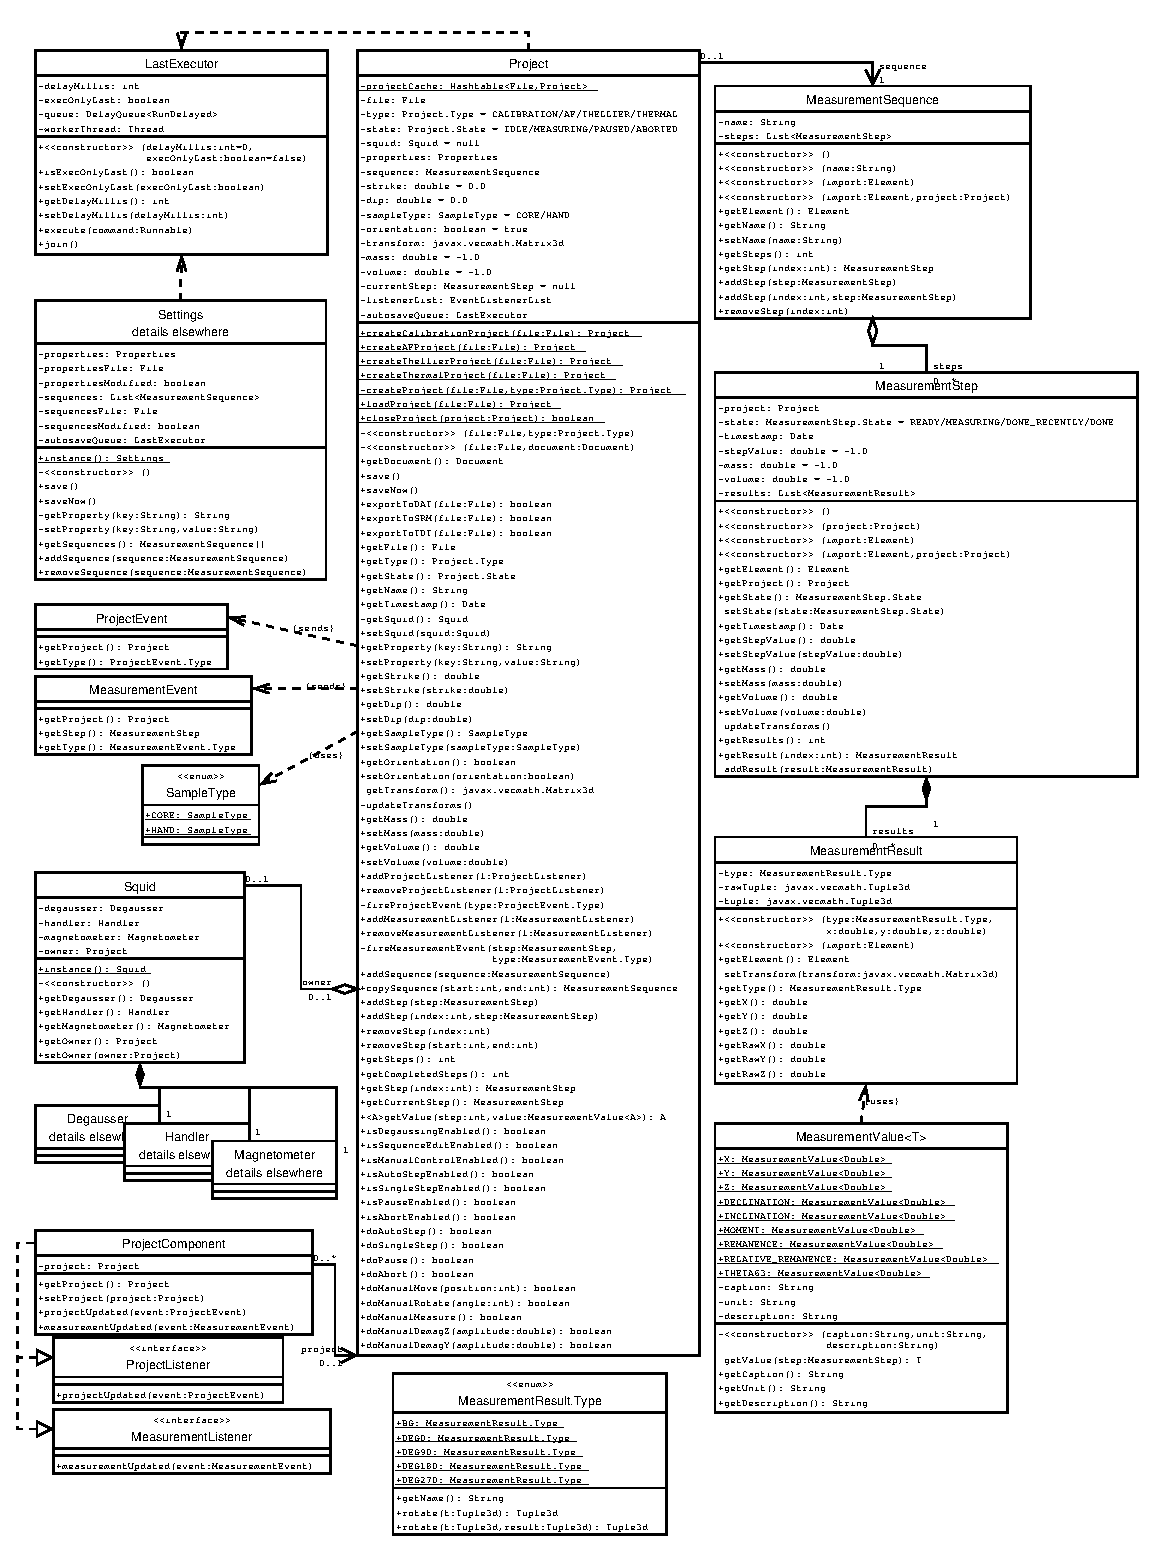
\includegraphics[width=17cm]{dia/core.eps}
\caption{Squid class diagram: data classes}
\label{fig:core}
\end{center}
\end{figure}

Class diagram of data classes is in Figure~\ref{fig:core}.

Data classes are in packages ikayaki, ikayaki.squid and ikayaki.util.

Package ikayaki holds generic data classes, ikayaki.squid holds classes loosely related to the squid interface, and ikayaki.util has utilities (\ref{sec:utilities}).

\subsubsection{Project data}

Responsible for holding all the measurement data and controlling the SQUID. Most of the GUI classes use the Project class. When the state of the project changes, the Project class fires ProjectEvents and MeasurementEvents to the GUI classes, which in turn will call the Project class to get the changed information.

The classes Project, MeasurementSequence, MeasurementStep, MeasurementResult and MeasurementValue are shown in Figure~\ref{fig:core}.

\subsubsection{Squid interface}
\insertdia{core-squid}

Squid Interface offers the Project class an interface to safely control the SQUID magnetometer. It holds three subclasses that handle communication to to three separate parts of the SQUID (Handler, Degausser and Magnetometer).

Classes are Squid, Handler, Magnetometer, Degausser.

\subsubsection{Squid emulator}
\insertdia{core-squidemu}

This is separate from other and is used only for testing the Squid Interface that it works correctly.

\subsubsection{Serial communication}
\insertdia{core-serial}

SerialIO and classes related to it takes care of the harware layer of serial communication. Using these classes Ikayaki communicates with the Degausser, Samplehandler and Magnetometer. SerialIO represents one serial port and when it's created it reserves the port to itself. SerialProperties class includes all the configuration data for the serial port.

\subsubsection{Global settings}

Global properties that are used all around the program. The Settings class provides a global point for retrieving and modifying the properties.

The class Settings is shown in Figure~\ref{fig:core} and details of all the properties are in the documentation.

\subsubsection{Utilities}
\label{sec:utilities}

Miscellaneous classes that are used nowhere in particular.


\subsection{GUI classes and methods}

\begin{figure}
\begin{center}
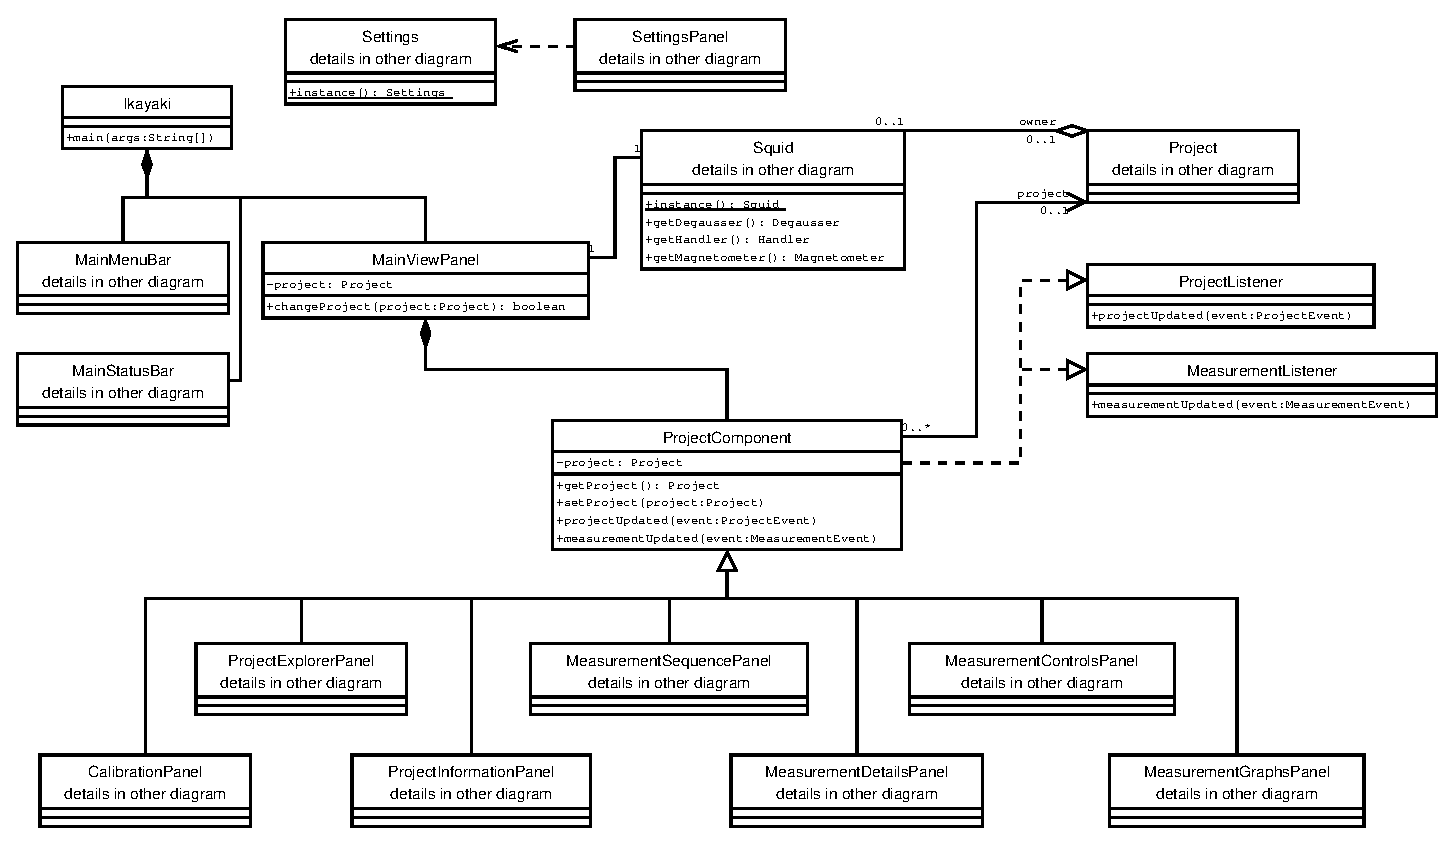
\includegraphics[angle=90,width=12cm]{dia/gui.eps}
\caption{Squid class diagram: GUI classes}
\label{fig:gui}
\end{center}
\end{figure}

Class diagram of gui classes is in Figure~\ref{fig:gui}. This section is divided into sections by gui components, each of which has one or more classes.

All gui classes are in package ikayaki.gui.

\subsubsection{Generic GUI components}

ProjectComponent, a generic gui base class which handles registering Project- and MeasurementListeners to new projects, and which every project-dependant gui component subclasses. See Figure~\ref{fig:core} and Figure~\ref{fig:gui}.

\subsubsection{Main window}
\insertdia{gui-main}

\subsubsection{Configuration window}

Separate window which is opened from menubar and it updates settings for Squid interface. Used usually only when system is installed to 
setup it.

\subsubsection{Project Explorer}
\insertdia{gui-explorer}

Located at middle left side of main window.

ProjectExplorerPanel handles loading existing projects and creating new ones. Shows a listing of project files in current directory, which can be changed by typing new directory into ComboBox text field, or using the browse-button and standars dir chooser dialog. ComboBox also holds directory history, and, when typing text into it's text field, automatically shows autocomplete results.

NewProjectPanel has components for creating a new project.

ProjectExplorerTable is a JTable with the project file listing, including "filename", "type" and "last modified" columns.

ProjectExplorerPopupMenu has options for exporting project files into different formats.

\subsubsection{Calibration}
\insertdia{gui-calibration}

Located at upper left corner of main window.

CalibrationPanel holds predefined "Holder noise" and "Standard sample" projects for calibration in a similar table as Project Explorer. Also has a "Calibrate" button, which executes selected calibration project, similarly to clicking "Single step" in normal projects.

\subsubsection{Project information}

Located at lower left corner of main window.

Contains and allows editing of basic inforamtion of sample.

\subsubsection{Sequence and measurement data}

Located at upper middle side of main window.

Contains and allows editing of measurement sequence. Whenever
measurement step is finished its data is added here.

\subsubsection{Measurement details}

Located at lower middle side of main window.

Contains details of ongoing measurement or row selected in measrurement sequence.

\subsubsection{Measurement controls}
\insertdia{gui-mcontrols}

Located at upper right corner of main window.

MeasurementControlsPanel holds the buttons for controlling measurements, a help picture for sample inserting, radiobuttons for changing +z/-z orientation of sample, magnetometer status picture and manual controlling components.

MagnetometerStatusPanel shows an image of current magnetometer status, as in sample holder position and rotation. Image is updated according to MeasurementEvents received.

ManualControlsPanel has controls for fully manual measuring, which are enabled when no "normal" measurements are happening.

\subsubsection{Graphs}
\insertdia{gui-graphs}

Graph panels visualize the measurement data. They are located at the lower right corner in the UI. MeasurementGraphsPanel listens to MeasurementEvents to update the measurement data in plots. AbstractPlot is an abstract class which implements all the general features of graph plots. IntensityPlot and StereoPlot extend the functionality of AbstractPlot and implement their special drawing features accordingly.


\section{Data classes and methods}
\label{sec:data}

\subsection{Project data}

\beginClass{Project}
\classPackage{ikayaki}
\classDeclaration{public class Project}
\classCreatedBy{ProjectExplorerPanel}
\classUses{MeasurementSequence}
\classUses{MeasurementStep}
\classUses{MeasurementResult}
\classUses{MeasurementValue}
\classUses{Squid}
\classUses{RunQueue}
\classUses{ProjectEvent}
\classUses{MeasurementEvent}
\classComment{
	Represents a measurement project file. Project is responsible for managing and storing the data that is recieved from the magnetometer measurements. Any changes made to the project will be written to file regularly (autosave).
	
	Project is responsible for controlling the magnetometer through the SQUID API. Controlling the SQUID will be done in a private worker thread. Only one project at a time may access the SQUID.
	
	All operations are thread-safe.
}
\classPatterns{Facade}
\classEvent{On property change}{Autosaving will be invoked and the project written to file after a short delay.}
\classEvent{On measurement started/ended/paused/aborted}{ProjectEvent will be fired to all project listeners.}
\classEvent{On measurement subphase started/completed}{MeasurementEvent will be fired to all measurement listeners.}
\classEvent{On declination/inclination/volume changed}{The updated transformation matrix will be applied to all measurements and a ProjectEvent will be fired to all project listeners.}
\closeClass

\beginField{projectCache}
\fieldDeclaration{private static Hashtable<File,Project> projectCache}
\fieldComment{
	Caches the created and loaded Project objects to make sure that no more than one object will be created for each physical file.
}
\closeField

\beginField{file}
\fieldDeclaration{private File file}
\fieldComment{
	Location of the project file in the local file system. Autosaving will save the project to this file.
}
\closeField

\beginField{type}
\fieldDeclaration{private Type type}
\fieldComment{
	Type of the measurement project. This will affect which features of the project are enabled and disabled.
}
\closeField

\beginField{state}
\fieldDeclaration{private State state}
\fieldValue{IDLE}
\fieldComment{
	Current state of the measurements. If no measurement is running, then state is IDLE. Only one measurement may be running at a time.
}
\closeField

\beginField{squid}
\fieldDeclaration{private Squid squid}
\fieldValue{null}
\fieldComment{
	Pointer to the SQUID device interface, or null if this project is not its owner.
}
\closeField

\beginField{properties}
\fieldDeclaration{private Properties properties}
\fieldComment{
	Custom properties of this project stored in a map. The project is not interested in what properties are stored; it only saves them.
}
\closeField

\beginField{sequence}
\fieldDeclaration{private MeasurementSequence sequence}
\fieldComment{
	Measurement sequence of this project. In the beginning are all completed measurement steps, and in the end are planned measurement steps. Completed measurements may NOT be deleted.
}
\closeField

\beginField{strike}
\fieldDeclaration{private double strike}
\fieldValue{0.0}
\fieldComment{
	Strike of the sample. Will be used to create the transform matrix.
}
\closeField

\beginField{dip}
\fieldDeclaration{private double dip}
\fieldValue{0.0}
\fieldComment{
	Dip of the sample. Will be used to create the transform matrix.
}
\closeField

\beginField{sampleType}
\fieldDeclaration{private SampleType sampleType}
\fieldValue{CORE}
\fieldComment{
	Type of the sample. Will be used to create the transform matrix.
}
\closeField

\beginField{transform}
\fieldDeclaration{private Matrix3d transform}
\fieldValue{new Matrix3d()}
\fieldComment{
	Matrix for correcting the sample's orientation. The matrix will be updated whenever the strike, dip or sampleType is changed. After that the updated matrix will be applied to all measurements.
}
\closeField

\beginField{mass}
\fieldDeclaration{private double mass}
\fieldValue{-1.0}
\fieldComment{
	Mass of the sample, or a negative value if no mass is defined.
}
\closeField

\beginField{volume}
\fieldDeclaration{private double volume}
\fieldValue{-1.0}
\fieldComment{
	Volume of the sample, or a negative value if no volume is defined.
}
\closeField

\beginField{currentStep}
\fieldDeclaration{private MeasurementStep currentStep}
\fieldValue{null}
\fieldComment{
	Current measurement step, or null if no measurement is running.
}
\closeField

\beginField{listenerList}
\fieldDeclaration{private EventListenerList listenerList}
\fieldValue{new EventListenerList()}
\fieldComment{
	Listeners for this project.
}
\closeField

\beginField{autosaveQueue}
\fieldDeclaration{private RunQueue autosaveQueue}
\fieldValue{new RunQueue(500, true)}
\fieldComment{
	Scheduler for automatically writing the modified project to file after a short delay.
}
\closeField

\beginMethod{createCalibrationProject(File)}
\methodDeclaration{public static Project createCalibrationProject(File file)}
\methodComment{
	Creates a calibration project file.
}
\methodParam{file}{path for the new project file.}
\methodReturn{the created project, or null if file was not writable.}
\closeMethod

\beginMethod{createAFProject(File)}
\methodDeclaration{public static Project createAFProject(File file)}
\methodComment{
	Creates an AF project file.
}
\methodParam{file}{path for the new project file.}
\methodReturn{the created project, or null if file was not writable.}
\closeMethod

\beginMethod{createThellierProject(File)}
\methodDeclaration{public static Project createThellierProject(File file)}
\methodComment{
	Creates a thellier project file.
}
\methodParam{file}{path for the new project file.}
\methodReturn{the created project, or null if file was not writable.}
\closeMethod

\beginMethod{createThermalProject(File)}
\methodDeclaration{public static Project createThermalProject(File file)}
\methodComment{
	Creates a thermal project file.
}
\methodParam{file}{path for the new project file.}
\methodReturn{the created project, or null if file was not writable.}
\closeMethod

\beginMethod{createProject(File,Type)}
\methodDeclaration{private static Project createProject(File file, Type type)}
\methodComment{
	Creates a project file of the specified type. Ensures that the project file has been written to disk. Adds the created Project object to projectCache.
}
\methodParam{file}{path for the new project file.}
\methodParam{type}{type of the project.}
\methodReturn{the created project, or null if file was not writable.}
\closeMethod

\beginMethod{loadProject(File)}
\methodDeclaration{public static Project loadProject(File file)}
\methodComment{
	Loads a saved project file. If the file has already been loaded, will return a reference to the existing Project object.
}
\methodParam{file}{project file to be loaded.}
\methodReturn{the loaded project, or null if file is not a valid project file or it was not readable.}
\closeMethod

\beginMethod{closeProject(Project)}
\methodDeclaration{public static boolean closeProject(Project project)}
\methodComment{
	Ensures that the project file is saved and frees the resources taken by the project. A project should not be used after it has been closed -- any further use of the object is undefined (probably will create NullPointerExceptions). The closed project is removed from the projectCache. A project can not be closed if it has a measurement running.
}
\methodParam{project}{project to be closed.}
\methodReturn{true if the project has been closed, false if a measurement is running and the project can not be closed.}
\methodThrows{NullPointerException}{if the project is null.}
\closeMethod

\beginMethod{Project(File,Type)}
\methodDeclaration{private Project(File file, Type type)}
\methodComment{
	Creates a new project of the specified type. This constructor will not write to file, so the user of this method should call the saveNow() method after the project is initialized.
}
\methodParam{file}{path for this project file. The file should exist (may be empty) and be writable, but this constructor will not check it.}
\methodParam{type}{type of the project.}
\methodReturn{the created project.}
\closeMethod

\beginMethod{Project(File,Document)}
\methodDeclaration{private Project(File file, Document document)}
\methodComment{
	Creates a new project from the specified document. This constructor will assume that the specified file is the same from which the document was read.
}
\methodParam{file}{path for this project file. The file should be the same from which document was read and be writable, but this constructor will not check it.}
\methodParam{document}{the document from which this project will be created.}
\methodReturn{the created project.}
\methodThrows{IllegalArgumentException}{if the document was not in the right format.}
\closeMethod

\beginMethod{getDocument()}
\methodDeclaration{public synchronized Document getDocument()}
\methodComment{
	Exports this project to a DOM document.
}
\closeMethod

\beginMethod{save()}
\methodDeclaration{public synchronized void save()}
\methodComment{
	Invokes autosaving. This method will schedule a saving operation and return. After this method has not been called for a short while, the project will be written to file.
}
\closeMethod

\beginMethod{saveNow()}
\methodDeclaration{public void saveNow()}
\methodComment{
	Writes this project to its project file and waits for the operation to complete.
	
	(NOTE: Synchronizing is done inside the method)
}
\methodThrows{IOException}{if there was an error when writing to file.}
\closeMethod

\beginMethod{getFile()}
\methodDeclaration{public synchronized File getFile()}
\methodComment{
	Returns the project file of this project.
}
\closeMethod

\beginMethod{getType()}
\methodDeclaration{public synchronized Type getType()}
\methodComment{
	Returns the type of this project.
}
\closeMethod

\beginMethod{getState()}
\methodDeclaration{public synchronized State getState()}
\methodComment{
	Returns the current measurement state of this project.
}
\closeMethod

\beginMethod{getName()}
\methodDeclaration{public synchronized String getName()}
\methodComment{
	Returns the name of this project. The name is equal to the name of the project file without the file extension.
}
\closeMethod

\beginMethod{getTimestamp()}
\methodDeclaration{public synchronized Date getTimestamp()}
\methodComment{
	Returns the timestamp of the last completed measurement. This is usually less than the last modified date of the file, because this is not affected by changing the project's properties.
}
\closeMethod

\beginMethod{getSquid()}
\methodDeclaration{private synchronized Squid getSquid()}
\methodComment{
	Returns the Squid if this project is its owner, otherwise returns null.
	
	(NOTE: Make this method public? Or return a Proxy (see design patterns), so others can know where the handler is moving but not control it?)
}
\closeMethod

\beginMethod{setSquid(Squid)}
\methodDeclaration{public synchronized boolean setSquid(Squid squid)}
\methodComment{
	Sets this project the owner of the Squid. Uses the setOwner() method of the specified Squid.
	
	Only one project may own the Squid at a time. The Squid must be first detached with "setSquid(null)" from its owner before it can be given to another project. Detaching the Squid is possible only when the project's state is IDLE.
}
\methodParam{squid}{pointer to the SQUID interface, or null to detach this project from it.}
\methodReturn{true if the operation was completed, false if the Squid has another owner or a measurement is running (in which case nothing was changed).}
\closeMethod

\beginMethod{getProperty(String)}
\methodDeclaration{public synchronized String getProperty(String key)}
\methodComment{
	Returns a project information property.
}
\methodParam{key}{the key which is associated with the property.}
\methodReturn{the specified property, or an empty String if the property is not set.}
\closeMethod

\beginMethod{setProperty(String,String)}
\methodDeclaration{public synchronized void setProperty(String key, String value)}
\methodComment{
	Sets a project information property.
}
\methodParam{key}{the key which is associated with the property.}
\methodParam{value}{new value for the property, or null to remove the property.}
\closeMethod

\beginMethod{getStrike()}
\methodDeclaration{public synchronized double getStrike()}
\methodComment{
	Returns the strike of the sample.
}
\closeMethod

\beginMethod{setStrike(double)}
\methodDeclaration{public synchronized void setStrike(double strike)}
\methodComment{
	Sets the strike of the sample and calls updateTransforms().
}
\closeMethod

\beginMethod{getDip()}
\methodDeclaration{public synchronized double getDip()}
\methodComment{
	Returns the dip of the sample.
}
\closeMethod

\beginMethod{setDip(double)}
\methodDeclaration{public synchronized void setDip(double dip)}
\methodComment{
	Sets the dip of the sample and calls updateTransforms().
}
\closeMethod

\beginMethod{getSampleType()}
\methodDeclaration{public synchronized SampleType getSampleType()}
\methodComment{
	Returns the type of the sample.
}
\closeMethod

\beginMethod{setSampleType(SampleType)}
\methodDeclaration{public synchronized void setSampleType(SampleType sampleType)}
\methodComment{
	Sets the type of the sample and calls updateTransforms().
}
\methodThrows{NullPointerException}{if sampleType is null.}
\closeMethod

\beginMethod{getTransform()}
\methodDeclaration{synchronized Matrix3d getTransform()}
\methodComment{
	Returns the current transformation matrix for the sample. For performance reasons, this method returns a reference to the internal data structure and not a copy of it.
	
	WARNING!!! Absolutely NO modification of the data contained in this matrix should be made -- if any such manipulation is necessary, it should be done on a copy of the matrix returned rather than the matrix itself.
}
\methodReturn{reference to the transformation matrix.}
\closeMethod

\beginMethod{updateTransforms()}
\methodDeclaration{private synchronized void updateTransforms()}
\methodComment{
	Recalculates the transformation matrix and updates all measurements. This method is called automatically by the setStrike(), setDip() and setSampleType() methods.
}
\closeMethod

\beginMethod{getMass()}
\methodDeclaration{public synchronized double getMass()}
\methodComment{
	Returns the mass of the sample.
}
\methodReturn{mass of the sample, or a negative number if no mass is specified.}
\closeMethod

\beginMethod{setMass(double)}
\methodDeclaration{public synchronized void setMass(double mass)}
\methodComment{
	Sets the mass of the sample.
}
\methodParam{mass}{mass of the sample, or a negative number to clear it.}
\closeMethod

\beginMethod{getVolume()}
\methodDeclaration{public synchronized double getVolume()}
\methodComment{
	Returns the volume of the sample.
}
\methodReturn{volume of the sample, or a negative number if no volume is specified.}
\closeMethod

\beginMethod{setVolume(double)}
\methodDeclaration{public synchronized void setVolume(double volume)}
\methodComment{
	Sets the volume of the sample.
}
\methodParam{volume}{volume of the sample, or a negative number to clear it.}
\closeMethod

\beginMethod{addProjectListener(ProjectListener)}
\methodDeclaration{public synchronized void addProjectListener(ProjectListener l)}
\methodComment{
	Adds a ProjectListener to the project.
}
\methodParam{l}{the listener to be added.}
\closeMethod

\beginMethod{removeProjectListener(ProjectListener)}
\methodDeclaration{public synchronized void removeProjectListener(ProjectListener l)}
\methodComment{
	Removes a ProjectListener from the project.
}
\methodParam{l}{the listener to be removed}
\closeMethod

\beginMethod{fireProjectEvent(ProjectEvent.Type)}
\methodDeclaration{private synchronized void fireProjectEvent(ProjectEvent.Type type)}
\methodComment{
	Notifies all listeners that have registered for ProjectEvents.
}
\methodParam{type}{type of the event.}
\closeMethod

\beginMethod{addMeasurementListener}
\methodDeclaration{public synchronized void addMeasurementListener(MeasurementListener l)}
\methodComment{
	Adds a MeasurementListener to the project.
}
\methodParam{l}{the listener to be added.}
\closeMethod

\beginMethod{removeMeasurementListener}
\methodDeclaration{public synchronized void removeMeasurementListener(MeasurementListener l)}
\methodComment{
	Removes a MeasurementListener from the project.
}
\methodParam{l}{the listener to be removed}
\closeMethod

\beginMethod{fireMeasurementEvent(MeasurementStep,MeasurementEvent.Type)}
\methodDeclaration{private synchronized void fireMeasurementEvent(MeasurementStep step, MeasurementEvent.Type type)}
\methodComment{
	Notifies all listeners that have registered for MeasurementEvents.
}
\methodParam{step}{the measurement step that has generated the event.}
\methodParam{type}{the type of the event.}
\closeMethod

\beginMethod{addSequence(MeasurementSequence}
\methodDeclaration{public synchronized void addSequence(MeasurementSequence sequence)}
\methodComment{
	Appends a sequence to this project's sequence. Only the stepValues will be copied from the specified sequence and added as new steps to this project.
	
	If isSequenceEditEnabled() is false, nothing will be done.
}
\methodParam{sequence}{the measurement sequence to be added.}
\methodThrows{NullPointerException}{if sequence is null.}
\closeMethod

\beginMethod{copySequence(int,int)}
\methodDeclaration{public synchronized MeasurementSequence copySequence(int start, int end)}
\methodComment{
	Returns a copy of this project's sequence. Only the stepValues will be copied from this project's sequence. The returned sequence will have no name.
}
\methodParam{start}{index of the first step in the sequence.}
\methodParam{end}{index of the last step in the sequence. If end < start, then an empty sequence will be returned.}
\methodReturn{copy of the sequence with only stepValues and no results.}
\methodThrows{IndexOutOfBoundsException}{if the index is out of range (start < 0 || end >= getSteps()).}
\closeMethod

\beginMethod{addStep(MeasurementStep)}
\methodDeclaration{public synchronized void addStep(MeasurementStep step)}
\methodComment{
	Appends a step to this project's sequence. Only the stepValue will be copied from the specified step and added as new steps to this project.
	
	If isSequenceEditEnabled() is false, nothing will be done.
}
\methodParam{step}{the measurement step to be added.}
\methodThrows{NullPointerException}{if step is null.}
\closeMethod

\beginMethod{addStep(int,MeasurementStep)}
\methodDeclaration{public synchronized void addStep(int index, MeasurementStep step)}
\methodComment{
	Adds a step to the specified index of this project's sequence. Only the stepValue will be copied from the specified step and added as new steps to this project.
	
	The index must be such, that the indices of the completed measurements will not change.
	
	If isSequenceEditEnabled() is false, nothing will be done.
}
\methodParam{index}{the index to which the step will be added.}
\methodParam{step}{the measurement step to be added.}
\methodThrows{IndexOutOfBoundsException}{if the index is out of range (index < getCompletedSteps() || index > getSteps()).}
\methodThrows{NullPointerException}{if step is null.}
\closeMethod

\beginMethod{removeStep(int)}
\methodDeclaration{public synchronized void removeStep(int index)}
\methodComment{
	Removes a step from this project's sequence. Completed measurements can not be removed.
	
	If isSequenceEditEnabled() is false, nothing will be done.
}
\methodParam{index}{the index of the step to be removed.}
\methodThrows{IndexOutOfBoundsException}{if the index is out of range (index < getCompletedSteps() || index >= getSteps()).}
\closeMethod

\beginMethod{removeStep(int,int)}
\methodDeclaration{public synchronized void removeStep(int start, int end)}
\methodComment{
	Removes a series of steps from this project's sequence. Completed measurements can not be removed.
	
	If isSequenceEditEnabled() is false, nothing will be done.
}
\methodParam{start}{the first index to be removed.}
\methodParam{end}{the last index to be removed. If end < start, no steps will be removed.}
\methodThrows{IndexOutOfBoundsException}{if the index is out of range (start < getCompletedSteps() || end >= getSteps()).}
\closeMethod

\beginMethod{getSteps()}
\methodDeclaration{public synchronized int getSteps()}
\methodComment{
	Returns the number of steps in this project.
}
\closeMethod

\beginMethod{getCompletedSteps()}
\methodDeclaration{public synchronized int getCompletedSteps()}
\methodComment{
	Returns the number of completed steps in this project. Steps that are currently being measured, are included in this count. Completed steps are always first in the sequence.
}
\closeMethod

\beginMethod{getStep(int)}
\methodDeclaration{public synchronized MeasurementStep getStep(int index)}
\methodComment{
	Returns a step from the sequence.
}
\methodParam{index}{the index of the step.}
\methodReturn{the specified step.}
\methodThrows{IndexOutOfBoundsException}{if the index is out of range (index < 0 || index >= getSteps()).}
\closeMethod

\beginMethod{getCurrentStep()}
\methodDeclaration{public synchronized MeasurementStep getCurrentStep()}
\methodComment{
	Returns the step that is currently being measured.
}
\methodReturn{the currently measured step, or null if no measurement is active.}
\closeMethod

\beginMethod{getValue(int,MeasurementValue)}
\methodDeclaration{public synchronized <A> A getValue(int step, MeasurementValue<A> algorithm)}
\methodComment{
	Calculates and returns a value from a measurement step. The specified MeasurementValue's algorithm will be used and the results returned.
}
\methodParam{step}{the measurement step from which the value is calculated.}
\methodParam{algorithm}{the algorithm for calculating the desired value.}
\methodReturn{the value returned by the algorithm, or null if it was not possible to calculate it.}
\methodThrows{NullPointerException}{if algorithm is null.}
\closeMethod

\beginMethod{isDegaussingEnabled()}
\methodDeclaration{public synchronized boolean isDegaussingEnabled()}
\methodComment{
	Tells whether it is allowed to use the degausser in this project. The returned value depends on the type and state of this project.
}
\closeMethod

\beginMethod{isSequenceEditEnabled()}
\methodDeclaration{public synchronized boolean isSequenceEditEnabled()}
\methodComment{
	Tells whether it is allowed to edit the sequence. The returned value depends on the type and state of this project.
}
\closeMethod

\beginMethod{isManualControlEnabled()}
\methodDeclaration{public synchronized boolean isManualControlEnabled()}
\methodComment{
	Tells whether it is allowed to control the Squid manually. The returned value depends on the type and state of this project.
}
\closeMethod

\beginMethod{isAutoStepEnabled()}
\methodDeclaration{public synchronized boolean isAutoStepEnabled()}
\methodComment{
	Tells whether it is allowed to do an auto step measurement. The returned value depends on the type and state of this project.
}
\closeMethod

\beginMethod{isSingleStepEnabled()}
\methodDeclaration{public synchronized boolean isSingleStepEnabled()}
\methodComment{
	Tells whether it is allowed to do a single step measurement. The returned value depends on the type and state of this project.
}
\closeMethod

\beginMethod{isPauseEnabled()}
\methodDeclaration{public synchronized boolean isPauseEnabled()}
\methodComment{
	Tells whether it is possible to pause the measurement. The returned value depends on the type and state of this project.
}
\closeMethod

\beginMethod{isAbortEnabled()}
\methodDeclaration{public synchronized boolean isAbortEnabled()}
\methodComment{
	Tells whether it is possible to abort the measurement. The returned value depends on the type and state of this project.
}
\closeMethod

\beginMethod{doAutoStep()}
\methodDeclaration{public synchronized boolean doAutoStep()}
\methodComment{
	Starts an auto step measurement. Will do nothing if isAutoStepEnabled() is false.
	
	The measurement will run in its own thread, and this method will not wait for it to finish.
}
\methodReturn{true if the measurement was started, otherwise false.}
\closeMethod

\beginMethod{doSingleStep()}
\methodDeclaration{public synchronized boolean doSingleStep()}
\methodComment{
	Starts a single step measurement. Will do nothing if isSingleStepEnabled() is false.
	
	The measurement will run in its own thread, and this method will not wait for it to finish.
}
\methodReturn{true if the measurement was started, otherwise false.}
\closeMethod

\beginMethod{doPause()}
\methodDeclaration{public synchronized boolean doPause()}
\methodComment{
	Pauses the currently running measurement. A paused measurement will halt after it finishes the current measurement step. Will do nothing if isPauseEnabled() is false.
	
	This method will notify the measurement thread to pause, but will not wait for it to finish.
}
\methodReturn{true if the measurement will pause, otherwise false.}
\closeMethod

\beginMethod{doAbort()}
\methodDeclaration{public synchronized boolean doAbort()}
\methodComment{
	Aborts the currently running measurement. An aborted measurement will halt immediately, leave the handler where it was and enable manual control. Will do nothing if isAbortEnabled() is false.
	
	This method will notify the measurement thread to abort, but will not wait for it to finish.
}
\methodReturn{true if the measurement will abort, otherwise false.}
\closeMethod


\beginClass{Project.Type}
\classPackage{ikayaki}
\classDeclaration{public enum Type}
\classComment{
	The type of the project. Options are CALIBRATION, AF, THELLIER and THERMAL.
}
\closeClass


\beginClass{Project.State}
\classPackage{ikayaki}
\classDeclaration{public enum State}
\classComment{
	The state of the project's measurements. Options are IDLE, MEASURING, PAUSED, ABORTED.
}
\closeClass


\beginClass{MeasurementSequence}
\classPackage{ikayaki}
\classDeclaration{public class MeasurementSequence}
\classCreatedBy{Project}
\classUses{MeasurementStep}
\classComment{
	A list of measurement steps. Steps can be added or removed from the sequence.
	
	All operations are thread-safe.
}
\closeClass

\beginField{name}
\fieldDeclaration{private String name}
\fieldValue{null}
\fieldComment{
	Name of the sequence or null if it has no name.
}
\closeField

\beginField{steps}
\fieldDeclaration{private List<MeasurementStep>}
\fieldValue{new ArrayList<MeasurementStep>()}
\fieldComment{
	The measurement steps of this sequence.
}
\closeField

\beginMethod{MeasurementSequence()}
\methodDeclaration{public MeasurementSequence()}
\methodComment{
	Creates an empty sequence with no name.
}
\methodReturn{the created sequence.}
\closeMethod

\beginMethod{MeasurementSequence(String)}
\methodDeclaration{public MeasurementSequence(String name)}
\methodComment{
	Creates an empty sequence with the specified name.
}
\methodParam{name}{name of the sequence.}
\methodReturn{the created sequence.}
\closeMethod

\beginMethod{MeasurementSequence(Element)}
\methodDeclaration{public MeasurementSequence(Element import)}
\methodComment{
	Creates a sequence from the specified element.
}
\methodParam{import}{the element from which this sequence will be created.}
\methodReturn{the created sequence.}
\methodThrows{IllegalArgumentException}{if the element was not in the right format.}
\closeMethod

\beginMethod{MeasurementSequence(Element,Project)}
\methodDeclaration{public MeasurementSequence(Element import, Project project)}
\methodComment{
	Creates a sequence from the specified element for a project.
}
\methodParam{import}{the element from which this sequence will be created.}
\methodParam{project}{the project whose sequence this will be. Needed for importing the measurement steps correctly.}
\methodReturn{the created sequence.}
\methodThrows{IllegalArgumentException}{if the element was not in the right format.}
\closeMethod

\beginMethod{getElement()}
\methodDeclaration{public synchronized Element getElement()}
\methodComment{
	Exports this sequence to a DOM element.
}
\closeMethod

\beginMethod{getName()}
\methodDeclaration{public synchronized String getName()}
\methodComment{
	Returns the name of this sequence.
}
\methodReturn{the name, or null if it has no name}
\closeMethod

\beginMethod{setName(String)}
\methodDeclaration{public synchronized void setName(String name)}
\methodComment{
	Sets the name of this sequence.
}
\closeMethod

\beginMethod{getSteps()}
\methodDeclaration{public synchronized int getSteps()}
\methodComment{
	Returns the number of steps in this sequence.
}
\closeMethod

\beginMethod{getStep(int)}
\methodDeclaration{public synchronized MeasurementStep getStep(int index)}
\methodComment{
	Returns the specified step from this sequence.
}
\methodParam{index}{the index of the step.}
\methodReturn{the specified step.}
\methodThrows{IndexOutOfBoundsException}{if the index is out of range (index < 0 || index >= getSteps()).}
\closeMethod

\beginMethod{addStep(MeasurementStep)}
\methodDeclaration{public synchronized void addStep(MeasurementStep step)}
\methodComment{
	Appends a step to this sequence.
}
\methodParam{step}{the measurement step to be added.}
\methodThrows{NullPointerException}{if step is null.}
\closeMethod

\beginMethod{addStep(int,MeasurementStep)}
\methodDeclaration{public synchronized void addStep(int index, MeasurementStep step)}
\methodComment{
	Adds a step to the specified index of this sequence.
}
\methodParam{index}{the index to which the step will be added.}
\methodParam{step}{the measurement step to be added.}
\methodThrows{IndexOutOfBoundsException}{if the index is out of range (index < 0 || index > getSteps()).}
\methodThrows{NullPointerException}{if step is null.}
\closeMethod

\beginMethod{removeStep(int)}
\methodDeclaration{public synchronized void removeStep(int index)}
\methodComment{
	Removes a step from this sequence.
}
\methodParam{index}{the index of the step to be removed.}
\methodThrows{IndexOutOfBoundsException}{if the index is out of range (index < 0 || index >= getSteps()).}
\closeMethod


\beginClass{MeasurementStep}
\classPackage{ikayaki}
\classDeclaration{public class MeasurementStep}
\classCreatedBy{Project, MeasurementSequencePanel}
\classUses{Project}
\classUses{MeasurementResult}
\classComment{
	A single step in a measurement sequence. Each step can include multiple measurements for improved precision. A step can have a different volume and mass than the related project, but by default the volume and mass of the project will be used. Only the project may change the state and results of a measurement step.
	
	All operations are thread-safe.
}
\closeClass

\beginField{project}
\fieldDeclaration{private Project project}
\fieldValue{null}
\fieldComment{
	The project that owns this step, or null if there is no owner.
}
\closeField

\beginField{state}
\fieldDeclaration{private State state}
\fieldValue{READY}
\fieldComment{
	Tells if this step has been completed or not, or if a measurement is still running.
}
\closeField

\beginField{timestamp}
\fieldDeclaration{private Date timestamp}
\fieldValue{null}
\fieldComment{
	The time the measurements were completed, or null if that has not yet happened.
}
\closeField

\beginField{stepValue}
\fieldDeclaration{private double stepValue}
\fieldValue{-1.0}
\fieldComment{
	The AF/Thermal value of this step, or a negative number if it has not been specified.
}
\closeField

\beginField{mass}
\fieldDeclaration{private double mass}
\fieldValue{-1.0}
\fieldComment{
	The mass of this step's sample, or a negative number to use the project's default mass.
}
\closeField

\beginField{volume}
\fieldDeclaration{private double volume}
\fieldValue{-1.0}
\fieldComment{
	The volume of this step's sample, or a negative number to use the project's default volume.
}
\closeField

\beginField{results}
\fieldDeclaration{private List<MeasurementResult> results}
\fieldValue{new ArrayList<MeasurementResult>()}
\fieldComment{
	The individual measurement results that are part of this measurement step.
}
\closeField

\beginMethod{MeasurementStep()}
\methodDeclaration{public MeasurementStep()}
\methodComment{
	Creates a blank measurement step.
}
\methodReturn{the created measurement step.}
\closeMethod

\beginMethod{MeasurementStep(Project)}
\methodDeclaration{public MeasurementStep(Project project)}
\methodComment{
	Creates a blank measurement step for a project.
}
\methodParam{project}{the project who is the owner of this step.}
\methodReturn{the created measurement step.}
\closeMethod

\beginMethod{MeasurementStep(Element)}
\methodDeclaration{public MeasurementStep(Element import)}
\methodComment{
	Creates a measurement step from the specified element.
}
\methodParam{import}{the element from which this step will be created.}
\methodReturn{the created measurement step.}
\methodThrows{IllegalArgumentException}{if the element was not in the right format.}
\closeMethod

\beginMethod{MeasurementStep(Element,Project)}
\methodDeclaration{public MeasurementStep(Element import, Project project)}
\methodComment{
	Creates a measurement step from the specified element for a project.
}
\methodParam{import}{the element from which this step will be created.}
\methodParam{project}{the project who is the owner of this step.}
\methodReturn{the created measurement step.}
\methodThrows{IllegalArgumentException}{if the element was not in the right format.}
\closeMethod

\beginMethod{getElement()}
\methodDeclaration{public synchronized Element getElement()}
\methodComment{
	Exports this step to a DOM element.
}
\closeMethod

\beginMethod{getProject()}
\methodDeclaration{public synchronized Project getProject()}
\methodComment{
	Returns the owner project of this step, or null if there is no owner.
}
\closeMethod

\beginMethod{getState()}
\methodDeclaration{public synchronized State getState()}
\methodComment{
	Tells if this step has been completed or not, or if a measurement is still running.
}
\closeMethod

\beginMethod{setState}
\methodDeclaration{void synchronized setState(State state)}
\methodComment{
	Sets the completion status of this step. Only the owner project may set the state.
}
\methodThrows{NullPointerException}{if state is null.}
\closeMethod

\beginMethod{getTimestamp()}
\methodDeclaration{public synchronized Date getTimestamp()}
\methodComment{
	Returns the time the measurements were completed, or null if that has not yet happened.
}
\closeMethod

\beginMethod{getStepValue()}
\methodDeclaration{public synchronized double getStepValue()}
\methodComment{
	Returns the AF/Thermal value of this step, or a negative number if it has not been specified.
}
\closeMethod

\beginMethod{setStepValue(double)}
\methodDeclaration{public synchronized void setStepValue(double stepValue)}
\methodComment{
	Sets the value of this step. A negative value will clear it.
}
\closeMethod

\beginMethod{getMass()}
\methodDeclaration{public synchronized double getMass()}
\methodComment{
	Returns the mass of this step's sample, or a negative number to use the project's default mass.
}
\closeMethod

\beginMethod{setMass(double)}
\methodDeclaration{public synchronized void setMass(double mass)}
\methodComment{
	Sets the mass of this step's sample. A negative value will clear it.
}
\closeMethod

\beginMethod{getVolume()}
\methodDeclaration{public synchronized double getVolume()}
\methodComment{
	Returns the volume of this step's sample, or a negative number to use the project's default volume.
}
\closeMethod

\beginMethod{setVolume(double)}
\methodDeclaration{public synchronized void setVolume(double volume)}
\methodComment{
	Sets the volume of this step's sample. A negative value will clear it.
}
\closeMethod

\beginMethod{updateTransforms()}
\methodDeclaration{synchronized void updateTransforms()}
\methodComment{
	Updates all of the measurement results with the owner project's transformation matrix.
}
\methodThrows{NullPointerException}{if this step is not owned by a project.}
\closeMethod

\beginMethod{getResults()}
\methodDeclaration{public synchronized int getResults()}
\methodComment{
	Returns the number of results in this step.
}
\closeMethod

\beginMethod{getResult(int)}
\methodDeclaration{public synchronized MeasurementResult getResult(int index)}
\methodComment{
	Returns a results from this step.
}
\methodParam{index}{the index of the result.}
\methodReturn{the specified result.}
\methodThrows{IndexOutOfBoundsException}{if the index is out of range (index < 0 || index >= getResults()).}
\closeMethod

\beginMethod{addResult(MeasurementResult)}
\methodDeclaration{public synchronized void addResult(MeasurementResult result)}
\methodComment{
	Appends a measurement result to this step. The transformation matrix of the result will be updated automatically.
}
\methodParam{result}{the result to be added.}
\methodThrows{NullPointerException}{if result is null.}
\closeMethod


\beginClass{MeasurementStep.State}
\classPackage{ikayaki}
\classDeclaration{public enum State}
\classComment{
	The state of a measurement step. Options are READY, MEASURING, DONE\_RECENTLY and DONE.
}
\closeClass


\beginClass{MeasurementResult}
\classPackage{ikayaki}
\classDeclaration{public class MeasurementResult}
\classCreatedBy{Magnetometer}
\classComment{
	A set of X, Y and Z values measured by the magnetometer. The raw XYZ values will be rotated in 3D space by using a transformation matrix. The project will set and update the transformation whenever its parameters are changed.
}
\closeClass

\beginField{type}
\fieldDeclaration{private Type type}
\fieldComment{
	The type of this result. Can be either a background noise measurement, or a sample in one of the four rotations.
}
\closeField

\beginField{rawTuple}
\fieldDeclaration{private Tuple3d rawTuple}
\fieldValue{new Tuple3d()}
\fieldComment{
	The unmodified measurements recieved from the squid.
}
\closeField

\beginField{tuple}
\fieldDeclaration{private Tuple3d tuple}
\fieldValue{new Tuple3d()}
\fieldComment{
	The measurements with the rotation and transformation matrix applied.
}
\closeField

\beginMethod{MeasurementResult(Type,double,double,double)}
\methodDeclaration{public MeasurementResult(Type type, double x, double y, double z}
\methodComment{
	Creates a new measurement result.
}
\methodParam{type}{the type (background or rotation) of this result.}
\methodParam{x}{the measured X coordinate value.}
\methodParam{y}{the measured Y coordinate value.}
\methodParam{z}{the measured Z coordinate value.}
\methodReturn{the created measurement result.}
\methodThrows{NullPointerException}{if type is null.}
\closeMethod

\beginMethod{MeasurementResult(Element)}
\methodDeclaration{public MeasurementResult(Element import)}
\methodComment{
	Creates a measurement result from the specified element. This will not apply the transformation matrix.
}
\methodParam{import}{the element from which this result will be created.}
\methodReturn{the created measurement result.}
\methodThrows{IllegalArgumentException}{if the element was not in the right format.}
\closeMethod

\beginMethod{getElement()}
\methodDeclaration{public Element getElement()}
\methodComment{
	Exports this result to a DOM element.
}
\closeMethod

\beginMethod{setTransform(Matrix3d)}
\methodDeclaration{void setTransform(Matrix3d transform)}
\methodComment{
	Applies a transformation matrix to this result.
}
\methodParam{transform}{the matrix to be applied.}
\methodThrows{NullPointerException}{if transform is null.}
\closeMethod

\beginMethod{getType()}
\methodDeclaration{public Type getType()}
\methodComment{
	Returns the type of this result (background or rotation).
}
\closeMethod

\beginMethod{getX()}
\methodDeclaration{public double getX()}
\methodComment{
	Returns the rotated and transformed X coordinate of this result.
}
\closeMethod

\beginMethod{getY()}
\methodDeclaration{public double getY()}
\methodComment{
	Returns the rotated and transformed Y coordinate of this result.
}
\closeMethod

\beginMethod{getZ()}
\methodDeclaration{public double getZ()}
\methodComment{
	Returns the rotated and transformed Z coordinate of this result.
}
\closeMethod

\beginMethod{getRawX()}
\methodDeclaration{public double getRawX()}
\methodComment{
	Returns the unmodified X coordinate of this result as recieved from the Squid.
}
\closeMethod

\beginMethod{getRawY()}
\methodDeclaration{public double getRawY()}
\methodComment{
	Returns the unmodified Y coordinate of this result as recieved from the Squid.
}
\closeMethod

\beginMethod{getRawZ()}
\methodDeclaration{public double getRawZ()}
\methodComment{
	Returns the unmodified Z coordinate of this result as recieved from the Squid.
}
\closeMethod


\beginClass{MeasurementResult.Type}
\classPackage{ikayaki}
\classDeclaration{public enum Type}
\classComment{
	The orientation of the sample when it was measured. Options are BG, DEG0, DEG90, DEG180 and DEG270.
}
\closeClass

\beginMethod{getName()}
\methodDeclaration{public String getName()}
\methodReturn{"BG", "0", "90", "180" or "270"}
\closeMethod

\beginMethod{rotate(Tuple3d)}
\methodDeclaration{public Tuple3d rotate(Tuple3d t)}
\methodComment{
	Rotates the raw XYZ values from the orientation of this object to that of DEG0. Rotating a BG or DEG0 will just copy the values directly.
}
\methodParam{t}{old values that need to be rotated.}
\methodReturn{a new object with the rotated values.}
\closeMethod

\beginMethod{rotate(Tuple3d,Tuple3d)}
\methodDeclaration{public Tuple3d rotate(Tuple3d t, Tuple3d result)}
\methodComment{
	Rotates the raw XYZ values from the orientation of this object to that of DEG0. Rotating a BG or DEG0 will just copy the values directly.
}
\methodParam{t}{old values that need to be rotated.}
\methodParam{result}{where the new values will be saved.}
\methodReturn{the same as the result parameter, or a new object if it was null.}
\closeMethod


\beginClass{MeasurementValue}
\classPackage{ikayaki}
\classDeclaration{public abstract class MeasurementValue<T>}
\classUses{MeasurementStep}
\classComment{
	Algorithms for calculating values from the measurements. A MeasurementValue object will be passed to the getValue() method of a project to retrieve the desired value.
}
\classPatterns{Strategy}
\closeClass

\beginField{X}
\fieldDeclaration{public static final MeasurementValue<Double> X}
\fieldComment{
	Calculates the average of all X components.
}
\closeField

\beginField{Y}
\fieldDeclaration{public static final MeasurementValue<Double> Y}
\fieldComment{
	Calculates the average of all Y components.
}
\closeField

\beginField{Z}
\fieldDeclaration{public static final MeasurementValue<Double> Z}
\fieldComment{
	Calculates the average of all Z components.
}
\closeField

\beginField{DECLINATION}
\fieldDeclaration{public static final MeasurementValue<Double> DECLINATION}
\fieldComment{
	Calculates the declination from the component averages.
}
\closeField

\beginField{INCLINATION}
\fieldDeclaration{public static final MeasurementValue<Double> INCLINATION}
\fieldComment{
	Calculates the inclination from the component averages.
}
\closeField

\beginField{MOMENT}
\fieldDeclaration{public static final MeasurementValue<Double> MOMENT}
\fieldComment{
	Calculates the length of the vector from the component averages.
}
\closeField

\beginField{REMANENCE}
\fieldDeclaration{public static final MeasurementValue<Double> REMANENCE}
\fieldComment{
	Calculates the remanence from the component averages and sample volume.
}
\closeField

\beginField{RELATIVE_REMANENCE}
\fieldDeclaration{public static final MeasurementValue<Double> RELATIVE\_REMANENCE}
\fieldComment{
	Calculates the remanence relative to the first measurement's remanence.
}
\closeField

\beginField{THETA63}
\fieldDeclaration{public static final MeasurementValue<Double> THETA63}
\fieldComment{
	Calculates the Theta 63 value from the measurement result set.
}
\closeField

\beginField{caption}
\fieldDeclaration{private String caption}
\fieldComment{
	A short name for the value.
}
\closeField

\beginField{unit}
\fieldDeclaration{private String unit}
\fieldComment{
	The unit of the value.
}
\closeField

\beginField{description}
\fieldDeclaration{private String description}
\fieldComment{
	A long description of the value.
}
\closeField

\beginMethod{MeasurementValue(String,String,String)}
\methodDeclaration{public MeasurementValue(String caption, String unit, String description)}
\methodComment{
	Creates a new measurement value.
}
\methodParam{caption}{a short name for the value.}
\methodParam{unit}{the unit of the value.}
\methodParam{description}{a long description of the value.}
\methodReturn{the created measurement value.}
\methodThrows{NullPointerException}{if any of the arguments is null.}
\closeMethod

\beginMethod{getValue(MeasurementStep)}
\methodDeclaration{abstract T getValue(MeasurementStep step)}
\methodComment{
	Calculates a specific value from a measurement step.
}
\methodParam{step}{the step from which the value will be calculated.}
\methodReturn{the calculated value, or null if it was not possible to calculate it.}
\methodThrows{NullPointerException}{if step is null.}
\closeMethod

\beginMethod{getCaption()}
\methodDeclaration{public String getCaption()}
\methodComment{
	Returns a short name for the value.
}
\closeMethod

\beginMethod{getUnit()}
\methodDeclaration{public String getUnit()}
\methodComment{
	Returns the unit of the value.
}
\closeMethod

\beginMethod{getDescription()}
\methodDeclaration{public String getDescription()}
\methodComment{
	Returns a long description of the value.
}
\closeMethod


\beginClass{ProjectEvent}
\classPackage{ikayaki}
\classDeclaration{public class ProjectEvent}
\classExtends{EventObject}
\classCreatedBy{Project}
\classComment{
	ProjectEvent is used to notify others about the state change of a project.
}
\closeClass

\beginField{project}
\fieldDeclaration{private Project project}
\fieldComment{
	The project that sent this event.
}
\closeField

\beginField{type}
\fieldDeclaration{private Type type}
\fieldComment{
	The type of event this is.
}
\closeField

\beginMethod{ProjectEvent(Project,Type)}
\methodDeclaration{public ProjectEvent(Project project, Type type)}
\methodComment{
	Creates a new project event.
}
\methodParam{project}{the project that sends this event.}
\methodParam{type}{the type of the event.}
\methodReturn{the created event.}
\methodThrows{NullPointerException}{if any of the arguments is null.}
\closeMethod

\beginMethod{getProject()}
\methodDeclaration{public Project getProject()}
\methodComment{
	Returns the project that sent this event.
}
\closeMethod

\beginMethod{getType()}
\methodDeclaration{public Type getType()}
\methodComment{
	Returns the type of this event.
}
\closeMethod


\beginClass{ProjectEvent.Type}
\classPackage{ikayaki}
\classDeclaration{public enum Type}
\classComment{
	The type of a project event. Options are STATE\_CHANGED, DATA\_CHANGED.
}
\closeClass


\beginClass{ProjectListener}
\classPackage{ikayaki}
\classDeclaration{public interface ProjectListener}
\classExtends{EventListener}
\classComment{
	Defines a listener for project events.
}
\closeClass

\beginMethod{projectUpdated(ProjectEvent)}
\methodDeclaration{public void projectUpdated(ProjectEvent event)}
\methodComment{
	Will be invoked whenever a project event happens.
}
\methodParam{event}{the event that happened.}
\closeMethod


\beginClass{MeasurementEvent}
\classPackage{ikayaki}
\classDeclaration{public class MeasurementEvent}
\classExtends{EventObject}
\classCreatedBy{Project}
\classComment{
	MeasurementEvent is used to notify listeners about the stages of an ongoing measurement.
}
\closeClass

\beginField{project}
\fieldDeclaration{private Project project}
\fieldComment{
	The project whose measurement sent this event.
}
\closeField

\beginField{step}
\fieldDeclaration{private MeasurementStep step}
\fieldComment{
	The measurement that sent this event.
}
\closeField

\beginField{type}
\fieldDeclaration{private Type type}
\fieldComment{
	The type of event this is.
}
\closeField

\beginMethod{MeasurementEvent(Project,MeasurementStep,Type)}
\methodDeclaration{public MeasurementEvent(Project project, MeasurementStep step, Type type)}
\methodComment{
	Creates a new measurement event.
}
\methodParam{project}{the project whose measurement sent this event.}
\methodParam{step}{the measurement that sent this event.}
\methodParam{type}{the type of event this is.}
\methodReturn{the created event.}
\methodThrows{NullPointerException}{if any of the arguments is null.}
\closeMethod

\beginMethod{getProject()}
\methodDeclaration{public Project getProject()}
\methodComment{
	Returns the project whose measurement sent this event.
}
\closeMethod

\beginMethod{getStep()}
\methodDeclaration{public MeasurementStep getStep()}
\methodComment{
	Returns the measurement that sent this event.
}
\closeMethod

\beginMethod{getType()}
\methodDeclaration{public Type getType()}
\methodComment{
	Returns the type of event this is.
}
\closeMethod


\beginClass{MeasurementEvent.Type}
\classPackage{ikayaki}
\classDeclaration{public enum Type}
\classComment{
	The type of a measurement event. Options are STEP\_START, STEP\_END, STEP\_ABORTED, HANDLER\_MOVE, HANDLER\_ROTATE, HANDLER\_STOP, DEMAGNETIZE\_START, DEMAGNETIZE\_END, VALUE\_MEASURED.
}
\closeClass


\beginClass{MeasurementListener}
\classPackage{ikayaki}
\classDeclaration{public interface MeasurementListener}
\classExtends{EventListener}
\classComment{
	Defines a listener for measurement events.
}
\closeClass

\beginMethod{measurementUpdated(MeasurementEvent)}
\methodDeclaration{public void measurementUpdated(MeasurementEvent event)}
\methodComment{
	Will be invoked whenever a measurement event happens.
}
\methodParam{event}{the event that happened.}
\closeMethod




\subsection{Squid interface}
\beginClass{Squid}
\classComment{
	Offers an interface for controlling the SQUID system. Reads settings from the Settings class. Creates instances of the degausser, handler and magnetometer interfaces and offers handlers for them.
}
\classPackage{ikayaki.squid}
\classDeclaration{public class Squid}
\classCreatedBy{MainViewPanel}
\classUses{Settings}
\classUses{Degausser}
\classUses{Handler}
\classUses{Magnetometer}
\classPatterns{Singleton}
\closeClass

\beginToc
\tocMethod{instance()}
\tocMethod{Squid()}
\tocMethod{getDegausser()}
\tocMethod{getHandler()}
\tocMethod{getMagnetometer()}
\tocMethod{updateSettings()}
\tocMethod{isOK()}
\tocMethod{setOwner(Project)}
\tocMethod{getOwner()}
\closeToc

\beginField{instance}
\fieldDeclaration{private static final Squid instance}
\fieldComment{Instance of the Squid interface.}
\closeField

\beginField{owner}
\fieldDeclaration{private Project owner}
\fieldComment{The project that is currently using the Squid, or null if no project is using it.}
\closeField

\beginField{degausser}
\fieldDeclaration{private final Degausser degausser}
\fieldComment{Instance of the degausser interface.}
\closeField

\beginField{handler}
\fieldDeclaration{private final Handler handler}
\fieldComment{Instance of the handler interface.}
\closeField

\beginField{magnetometer}
\fieldDeclaration{private final Magnetometer magnetometer}
\fieldComment{Instance of the magnetometer interface.}
\closeField

\beginMethod{instance()}
\methodDeclaration{public static synchronized Squid instance()}
\methodComment{
	Returns a reference to the Squid. If it has not yet been created, will create one.
}
\closeMethod

\beginMethod{Squid()}
\methodDeclaration{private Squid()}
\methodComment{
    Initializes the Squid interface. Creates instances of Degausser, Handler and Magnetometer.
}
\closeMethod

\beginMethod{getDegausser()}
\methodDeclaration{public Degausser getDegausser()}
\methodComment{
    Returns an interface for controlling the degausser.
}
\methodReturn{Handler for Degausser if available}
\closeMethod

\beginMethod{getHandler()}
\methodDeclaration{public Handler getHandler()}
\methodComment{
    Returns an interface for controlling the handler.
}
\methodReturn{Handler for Handler if available}
\closeMethod

\beginMethod{getMagnetometer()}
\methodDeclaration{public Magnetometer getMagnetometer()}
\methodComment{
    Returns an interface for controlling the magnetometer.
}
\methodReturn{Handler for Magnetometer if available}
\closeMethod

\beginMethod{updateSettings()}
\methodDeclaration{public synchronized void updateSettings()}
\methodComment{
    Checks which settings have changed and updates all the device interfaces. This method should be called when changes are made to the device parameters.
    
    This method starts a worker thread that will update the settings. If the current project has a measurement running, the thread will keep on retrying until the measurement is finished. Multiple calls to this method within a short period of time will update the settings only once.
}
\closeMethod

\beginMethod{isOK()}
\methodDeclaration{public synchronized boolean isOK()}
\methodComment{
    Checks whether all devices are working correctly.
}
\methodReturn{true if everything is correct, otherwise false.}
\closeMethod

\beginMethod{setOwner(Project)}
\methodDeclaration{public synchronized boolean setOwner(Project owner)}
\methodComment{
	Sets the owner of the Squid. Only one project may have access to the Squid at a time. This method may be called only from the Project class.
}
\methodParam{owner}{the project that will have exclusive access to the Squid.}
\methodReturn{true if successful, false if the existing owner had a running measurement.}
\closeMethod

\beginMethod{getOwner()}
\methodDeclaration{public synchronized Project getOwner()}
\methodComment{
    Returns project that is currently using the Squid.
}
\methodReturn{the project, or null if none is using the Squid.}
\closeMethod


\beginClass{Degausser}
\classComment{
    Offers an interface for controlling the degausser (demagnetizer). Because the data link is implemented in the degausser by a single board computer running a small basic program, the response time of the degausser to commands is slow. This class will make sure that commands are not sent faster than the device can handle.
}
\classPackage{ikayaki.squid}
\classDeclaration{public class Degausser}
\classImplements{SerialIOListener}
\classCreatedBy{Squid}
\classUses{Settings}
\classUses{SerialIO}
\classEvent{On new IO message}{reads the message and puts it in a buffer}
\closeClass

\beginToc
\tocMethod{Degausser()}
\tocMethod{updateSettings()}
\tocMethod{setCoil(char)}
\tocMethod{setAmplitude(int)}
\tocMethod{executeRampUp()}
\tocMethod{executeRampDown()}
\tocMethod{executeRampCycle()}
\tocMethod{demagnetize(int,char)}
\tocMethod{getStatus()}
\tocMethod{isOK()}
\closeToc

\beginField{messageBuffer}
\fieldDeclaration{private Stack messageBuffer}
\fieldComment{buffer for incoming messages, readed when needed.}
\closeField

\beginField{status}
\fieldDeclaration{private String status}
\fieldComment{Degaussers current status}
\closeField

\beginField{serialIO}
\fieldDeclaration{private SerialIO serialIO}
\fieldComment{COM port for communication.}
\closeField

\beginField{degausserCoil}
\fieldDeclaration{private int degausserCoil}
\fieldComment{(X, Y, Z) = (0,1,2) default axis Z}
\closeField

\beginField{degausserAmplitude}
\fieldDeclaration{private int degausserAmplitude}
\fieldComment{0->3000 default amp 0}
\closeField

\beginField{degausserDelay}
\fieldDeclaration{private int degausserDelay}
\fieldComment{1-9 seconds default delay 1 second}
\closeField

\beginField{degausserRamp}
\fieldDeclaration{private int degausserRamp}
\fieldComment{(3, 5, 7, 9) default 3}
\closeField

\beginField{degausserStatus}
\fieldDeclaration{private char degausserRamp}
\fieldComment{Z=Zero, T=Tracking, ?=Unknown}
\closeField

\beginMethod{Degausser()}
\methodDeclaration{public Degausser()}
\methodComment{
    Creates a new degausser interface. Opens connection to degausser COM port (if not open yet) and reads settings from the Setting class.
}
\closeMethod

\beginMethod{updateSettings()}
\methodDeclaration{public void updateSettings()}
\methodComment{
    Checks which settings have changed and updates the degausser interface. This method will be called by the Squid class.
}
\closeMethod

\beginMethod{setCoil(char)}
\methodDeclaration{private void setCoil(char coil)}
\methodComment{
    Sets coil X,Y,Z.
}
\methodParam{coil}{coil to set on.}
\closeMethod

\beginMethod{setAmplitude(int)}
\methodDeclaration{private void setAmplitude(int amplitude)}
\methodComment{
    Sets amplitude to ramp, range 0 to 3000.
}
\methodParam{amplitude}{amplitude to demag.}
\closeMethod

\beginMethod{executeRampUp()}
\methodDeclaration{private void executeRampUp()}
\methodComment{
    Performs Ramp up.
}
\closeMethod

\beginMethod{executeRampDown()}
\methodDeclaration{private void executeRampDown()}
\methodComment{
    Brings Ramp down.
}
\closeMethod

\beginMethod{executeRampCycle()}
\methodDeclaration{private void executeRampCycle()}
\methodComment{
    Performs Ramp up and down.
}
\closeMethod

\beginMethod{demagnetize(int,char)}
\methodDeclaration{public boolean demagnetize(int amplitude,char coil)}
\methodComment{
    Performs full sequence to demagnetize selected coil with the given amplitude. Blocking method.
}
\methodParam{amplitude}{amplitude to demag.}
\methodParam{coil}{coil to demagnetize. x,y or z}
\methodReturn{true if process was sended succesfully, otherwise false.}
\closeMethod

\beginMethod{getStatus()}
\methodDeclaration{public String getStatus()}
\methodComment{
    Gives configuration and ramp status.
}
\closeMethod

\beginMethod{isOK()}
\methodDeclaration{public boolean isOK()}
\methodComment{
    Checks if connection is ok.
}
\methodReturn{true if ok.}
\closeMethod


\beginClass{Handler}
\classComment{
    Offers an interface for controlling the sample handler.
}
\classPackage{ikayaki.squid}
\classDeclaration{public class Handler}
\classImplements{SerialIOListener}
\classCreatedBy{Squid}
\classUses{Settings}
\classUses{SerialIO}
\classEvent{On new IO message}{reads message and puts it in a buffer}
\closeClass

\beginToc
\tocMethod{Handler()}
\tocMethod{updateSettings()}
\tocMethod{getStatus()}
\tocMethod{isOK()}
\tocMethod{moveToHome()}
\tocMethod{moveToDegausser(char)}
\tocMethod{moveToMeasurement()}
\tocMethod{moveToBackground()}
\tocMethod{moveToPos(int)}
\tocMethod{stop()}
\tocMethod{rotateTo(int)}
\tocMethod{setOnline()}
\tocMethod{setAcceleration(int)}
\tocMethod{setDeceleration(int)}
\tocMethod{setBaseSpeed(int)}
\tocMethod{setVelocity(int)}
\tocMethod{setHoldTime(int)}
\tocMethod{setCrystalFrequence(int)}
\tocMethod{stopExecution()}
\tocMethod{performSlew()}
\tocMethod{setMotorPositive()}
\tocMethod{setMotorNegative()}
\tocMethod{setSteps(int)}
\tocMethod{setPosition(int)}
\tocMethod{go()}
\tocMethod{join()}
\tocMethod{verify(char)}
\tocMethod{setPositionRegister(int)}
\tocMethod{pollMessage()}
\closeToc

\beginField{messageBuffer}
\fieldDeclaration{private Stack messageBuffer}
\fieldComment{Buffer for incoming messages, readed when needed.}
\closeField

\beginField{status}
\fieldDeclaration{private String status}
\fieldComment{Handlers current status.}
\closeField

\beginField{serialIO}
\fieldDeclaration{private SerialIO serialIO}
\fieldComment{COM port for communication.}
\closeField

\beginField{acceleration}
\fieldDeclaration{private int acceleration}
\fieldComment{Value between 0 and 127 default 5. Settings in the
20-50 range are usually employed.}
\closeField

\beginField{deceleration}
\fieldDeclaration{private int deceleration}
\fieldComment{Value between 0 and 127 default 10. Settings in the
20-50 range are usually employed.}
\closeField

\beginField{velocity}
\fieldDeclaration{private int velocity}
\fieldComment{Value between 50 and 12 000. The
decimal number issued is 10 times the actual pulse rate to the motor. Since the
motor requires 200 pulses (full step) or 400 pulses (half step) per revolution,
a speed setting of M10000 sets the motor to revolve at 5 revolutions per second
in full step or 2.5 revolutions in half step. This rate is one-half the sample
rate rotation due to the pulley ratios. The sample handler is set up at the
factory for half stepping.}
\closeField

\beginField{measurementVelocity}
\fieldDeclaration{private int measurementVelocity}
\fieldComment{Speed in measurement, should be small.}
\closeField

\beginField{handlerStatus}
\fieldDeclaration{private String handlerStatus}
\fieldComment{5 end of move, previous G command complete, 7 hard limit stop, G motor is currently indexing.}
\closeField

\beginField{currentPosition}
\fieldDeclaration{private int currentPosition}
\fieldComment{Value between 1 and 16,777,215.}
\closeField

\beginField{homePosition}
\fieldDeclaration{private int homePosition}
\fieldComment{Value between 1 and 16,777,215.}
\closeField

\beginField{transverseYAFPosition}
\fieldDeclaration{private int transverseYAFPosition}
\fieldComment{AF demag position for transverse.}
\closeField

\beginField{axialAFPosition}
\fieldDeclaration{private int axialAFPosition}
\fieldComment{Axial AF demag position in steps, must be divisible by 10. Relative to Home.}
\closeField

\beginField{backgroundPosition}
\fieldDeclaration{private int backgroundPosition}
\fieldComment{Position in steps, must be divisible by 10. Relative to Home.}
\closeField

\beginField{measurementPosition}
\fieldDeclaration{private int measurementPosition}
\fieldComment{Position in steps, must be divisible by 10. Relative to Home.}
\closeField

\beginField{currentRotation}
\fieldDeclaration{private int currentRotation}
\fieldComment{Angles are between 0 (0) and 2000 (360).}
\closeField

\beginMethod{Handler()}
\methodDeclaration{public Handler()}
\methodComment{
    Creates a new handler interface. Opens connection to handler COM port and reads settings from the Settings class.
}
\closeMethod

\beginMethod{updateSettings()}
\methodDeclaration{public void updateSettings()}
\methodComment{
    Checks which settings have changed and updates the handler interface. This method will be called by the Squid class.
}
\closeMethod

\beginMethod{getStatus()}
\methodDeclaration{public String getStatus()}
\methodComment{
    Returns current status on Sample Handler: Position, rotation and moving status(stopped, on move).
}
\closeMethod

\beginMethod{isOK()}
\methodDeclaration{public boolean isOK()}
\methodComment{
    checks if connection is ok.
}
\methodReturn{True if ok}
\closeMethod

\beginMethod{moveToHome()}
\methodDeclaration{public void moveToHome()}
\methodComment{
    Commands the holder to move to home position.
}
\closeMethod

\beginMethod{moveToDegausser(char)}
\methodDeclaration{public void moveToDegausser(char position)}
\methodComment{
    Commands the holder to move to degauss position.
}
\methodParam{position}{tells which position to translate handler (x,y,z)}
\closeMethod

\beginMethod{moveToMeasurement()}
\methodDeclaration{public void moveToMeasurement()}
\methodComment{
   Commands the holder to move to measure position.
}
\closeMethod

\beginMethod{moveToBackground()}
\methodDeclaration{public void moveToBackground()}
\methodComment{
   Commands the holder to move to background position.
}
\closeMethod

\beginMethod{moveToPos(int)}
\methodDeclaration{public boolean moveToPos(int pos)}
\methodComment{
    Commands the holder to move to the specified position. Value must be between 1 and 16,777,215. Return true if good pos-value and moves handler there.
}
\methodParam{pos}{the position where the handler will move to.}
\methodReturn{true if given position was ok, otherwise false.}
\closeMethod

\beginMethod{stop()}
\methodDeclaration{public void stop()}
\methodComment{
    Commands the handler to stop its current job.
}
\closeMethod

\beginMethod{rotateTo(int)}
\methodDeclaration{public void rotateTo(int angle)}
\methodComment{
    Rotates the handler to the specified angle.
}
\methodParam{angle}{the angle in degrees to rotate the handler to.}
\closeMethod

\beginMethod{setOnline()}
\methodDeclaration{private void setOnline()}
\methodComment{
    Sends message to handler go online (@0).
}
\closeMethod

\beginMethod{setAcceleration(int)}
\methodDeclaration{private void setAcceleration(int a)}
\methodComment{
    Sends message to handler to set acceleration (Aa).
}
\methodParam{a}{Acceleration is a number from 0 to 127}
\closeMethod

\beginMethod{setDeceleration(int)}
\methodDeclaration{private void setDeceleration(int d)}
\methodComment{
    Sends message to handler to set deceleration (Dd).
}
\methodParam{a}{Deceleration is a number from 0 to 127}
\closeMethod

\beginMethod{setBaseSpeed(int)}
\methodDeclaration{private void setBaseSpeed(int b)}
\methodComment{
    Sends message to handler to set base speed. Base rate is the speed at which the motor motion starts and stops. (Bb).
}
\methodParam{b}{Base Speed is pulses per second and has a range of 50 to 5000.}
\closeMethod

\beginMethod{setVelocity(int)}
\methodDeclaration{private void setVelocity(int v)}
\methodComment{
    Sends message to handler to set maximum velocity (Mv).
}
\methodParam{v}{Velocity range is 50 to 20,000}
\closeMethod

\beginMethod{setHoldTime(int)}
\methodDeclaration{private void setHoldTime(int h)}
\methodComment{
    This command causes the POWER pin to be pulled low within a specified number of ticks after a move of the motor is completed and it will stay low until just prior to the start of the next move command. This command allows the holding torque of the motor to be turned off automatically after a delay for the mechanical system stabilize thus reducing power consumption and allowing the motor to be turned by hand if this feature is required. If the value is zero then the power is left on forever. (CH h).
}
\methodParam{h}{value from 0 to 127 representing the number of clock ticks to leave power on the motor after a move.}
\closeMethod

\beginMethod{setCrystalFrequence(int)}
\methodDeclaration{private void setCrystalFrequence(int cf)}
\methodComment{
    numbers. The crystal frequency is used by the chip for setting the base speed and maximum speed and for controlling the time for the wait command. (CX cf).
}
\methodParam{cf}{frequence range is 4,000,000 to 8,000.000}
\closeMethod

\beginMethod{stopExecution()}
\methodDeclaration{private void stopExecution()}
\methodComment{
    This command stops execution of the internal program if it is used in the program. If the motor is indexing it will ramp down and then stop. Use this command to stop the motor after issuing a slew command. (Q).
}
\closeMethod

\beginMethod{performSlew()}
\methodDeclaration{private void performSlew()}
\methodComment{
   Slew the motor up to maximum speed and continue until reaching a hard limit switch or receiving a quit (Q) command. (S).
}
\closeMethod

\beginMethod{setMotorPositive()}
\methodDeclaration{private void setMotorPositive()}
\methodComment{
   Set the motor direction of movement to positive. (+).
}
\closeMethod

\beginMethod{setMotorNegative()}
\methodDeclaration{private void setMotorNegative()}
\methodComment{
   Set the motor direction of movement to negative. (-).
}
\closeMethod

\beginMethod{setSteps(int)}
\methodDeclaration{private void setSteps(int s)}
\methodComment{
   Set the number of steps to move for the G command. (N s).
}
\methodParam{s}{steps range is 0 to 16,777,215}
\closeMethod

\beginMethod{setPosition(int)}
\methodDeclaration{private void setPosition(int p)}
\methodComment{
   Set absolute position to move for the G command. (P p).
}
\methodParam{p}{position range is 0 to 16,777,215}
\closeMethod

\beginMethod{go()}
\methodDeclaration{private void go()}
\methodComment{
   Send handler on move (G).
}
\closeMethod

\beginMethod{join()}
\methodDeclaration{private void join()}
\methodComment{
   Wait for handler to be idle. Blocking (F). Without the this command the SMC25 (Handler system) will continue to accept commands while the motor is moving. This may be desirable, as when changing speed during a move or working with the inputs or outputs. Or it may be undesirable, such as when you wish to make a series of indexes. Without the this command any subsequent Go commands received while the motor is indexing would set the "Not allowed while moving" message. Caution: If this command is used while the motor is executing a Slew command the only way to stop is with a reset or a hard limit switch input.
}
\closeMethod

\beginMethod{verify(char)}
\methodDeclaration{private String verify(char v)}
\methodComment{
   Gives result for wanted registery. (V v).
}
\methodParam{v}{A Acceleration

B Base speed

D Deceleration

E Internal program

G Steps remaining in current move. Zero if not indexing.

H Hold time

I Input pins

J Slow jog speed

M Maximum speed

N Number of steps to index

O Output pins

P Position. If motor is indexing this returns the position at the end of the index.

R Internal program pointer used by trace (T) or continue (X) commands. Also updated by enter (E) command.

W Ticks remaining on wait counter

X Crystal frequency
}
\methodReturn{returns registery as string}
\closeMethod

\beginMethod{setPositionRegister(int)}
\methodDeclaration{private void setPositionRegister(int r)}
\methodComment{
   Set the position register. This command sets the internal absolute position counter to the value of r. (Z r).
}
\methodParam{r}{position range is 0 to 16,777,215}
\closeMethod

\beginMethod{pollMessage()}
\methodDeclaration{private char pollMessage()}
\methodComment{
   Poll the device for any waiting messages such as errors or end of move. (%).
}
\methodReturn{0 Normal, no service required

1 Command error, illegal command sent

2 Range error, an out of range numeric parameter was sent

3 Command invalid while moving (e.g. G, S, H)

4 Command only valid in program (e.g. I, U, L)

5 End of move notice, a previous G command is complete

6 End of wait notice, a previous W command is complete

7 Hard limit stop, the move was stopped by the hard limit

8 End of program notice, internal program has completed

G Motor is indexing and no other notice pending
}
\closeMethod


\beginClass{Magnetometer}
\classComment{
	Offers an interface for controlling the magnetometer.
	
	Commands are at most five characters in length including a carriage return <CR>. The syntax is as follows: "<device><command><subcommand><data><CR>"
}
\classPackage{ikayaki.squid}
\classDeclaration{public class Magnetometer}
\classImplements{SerialIOListener}
\classCreatedBy{Squid}
\classUses{Settings}
\classUses{SerialIO}
\classEvent{On new IO message}{reads the message and puts it in a buffer}
\closeClass

\beginToc
\tocMethod{Magnetometer()}
\tocMethod{updateSettings()}
\tocMethod{reset(char)}
\tocMethod{resetCounter(char)}
\tocMethod{configure(char,char,char)}
\tocMethod{latchAnalog(char)}
\tocMethod{latchCounter(char)}
\tocMethod{getData(char,char,String)}
\tocMethod{openLoop(char)}
\tocMethod{clearFlux(char)}
\tocMethod{join()}
\tocMethod{readData()}
\tocMethod{getStatus()}
\tocMethod{isOK()}
\closeToc

\beginField{messageBuffer}
\fieldDeclaration{private Stack messageBuffer}
\fieldComment{Buffer for incoming messages, readed when needed.}
\closeField

\beginField{status}
\fieldDeclaration{private String status}
\fieldComment{Magnetometer's current status.}
\closeField

\beginField{serialIO}
\fieldDeclaration{private SerialIO serialIO}
\fieldComment{COM port for communication.}
\closeField

\beginMethod{Magnetometer()}
\methodDeclaration{public Magnetometer()}
\methodComment{
    Creates a new magnetometer interface. Opens connection to Magnetometer COM port (if its not open already) and reads settings from the Setting class.
}
\closeMethod

\beginMethod{updateSettings()}
\methodDeclaration{public void updateSettings()}
\methodComment{
    Checks which settings have changed and updates the magnetometer interface. This method will be called by the Squid class.
}
\closeMethod

\beginMethod{reset(char)}
\methodDeclaration{private String reset(char axis)}
\methodComment{
   Reset settings for axis.
}
\methodParam{axis}{x,y,x or a (all)}
\closeMethod

\beginMethod{resetCounter(char)}
\methodDeclaration{private void resetCounter(char axis)}
\methodComment{
   Reset counter for axis.
}
\methodParam{axis}{x,y,x or a (all)}
\closeMethod

\beginMethod{configure(char,char,char)}
\methodDeclaration{private void configure(char axis, char subcommand, char option)}
\methodComment{Used for configuring Magnetometer parameters. See subcommand for usages.}
\methodParam{axis}{x,y,x or a (all)}
\methodParam{subcommand}{The CONFIGURE subcommands follow: "F" Set filter configuration. The data subfield sets the filter to the indicated range. The four possible data values are: "1" One Hertz Filter; 1 Hz "T" Ten Hertz Filter; 10 Hz "H" One hundred Hertz Filter; 100 Hz "W" Wide band filter; WB "R" Set DC SQUID electronic range. The data subfield selects the range desired. The four possible data values are: "1" One time range; 1x "T" Ten times range; 10x "H" One hundred times range; 100x "E" Extended range; 1000x "S" Set/Reset the fast-slew option. Two data values are possible: "E" Enable the fast-slew; turn it on. "D" Disable the fast-slew; turn it off. "L" This subcommand opens or closes the SQUID feedback loop or resets the analog signal to +/- 1/2 flux quantum about zero. The three possible data values are: "O" Open the feedback loop. (This command also zeros the flux counter) "C" Close the feedback loop. "P" Pulse-reset (open then close) the feedback loop. (This command also zeros the flux counter)}
\methodParam{option}{see data values from subcommands.}
\closeMethod

\beginMethod{latchAnalog(char)}
\methodDeclaration{private void latchAnalog(char axis)}
\methodComment{
    axis is x,y,x or a (all).
}
\methodParam{axis}{x,y,x or a (all)}
\closeMethod

\beginMethod{latchCounter(char)}
\methodDeclaration{private void latchCounter(char axis)}
\methodComment{
    axis is x,y,x or a (all).
}
\methodParam{axis}{x,y,x or a (all)}
\closeMethod

\beginMethod{getData(char,char,String)}
\methodDeclaration{private String getData(char axis, char command, String datavalues)}
\methodComment{
	Generic send message sender, use with caution and knowledge. Checks if commands are good.
}
\methodParam{axis}{x,y,x}
\methodParam{command}{"D" Send back the analog data last captured with the LATCH command. The <data> field is not required. "C" Send back the counter value last captured with the LATCH command. The <data> field is not required. "S" Send back status. Various pieces of status can be sent by the magnetometer electronics.}
\methodParam{datavalues}{Datavalues one or more: "A" Send back all status. "F" Send back all filter status. "R" Send back all range status. "S" Send back slew status. "L" Send back SQUID feedback loop status. Return feedback, waiting time?}
\methodReturn{Returns data wanted, see command and datavalue}
\closeMethod

\beginMethod{openLoop(char)}
\methodDeclaration{public void openLoop(char axis)}
\methodComment{
   Pulse reset and opens feedback loop for axis. Need to be done to all axes before measuring.
}
\methodParam{axis}{x,y,x or a (all).}
\closeMethod

\beginMethod{clearFlux(char)}
\methodDeclaration{public void clearFlux(char axis)}
\methodComment{
    Clears flux counter for axis. Need to be done to all axes before measuring.
}
\methodParam{axis}{x,y,x or a (all).}
\closeMethod

\beginMethod{join()}
\methodDeclaration{public void join()}
\methodComment{
    Waits for magnetometer to settle down. Blocking.
}
\closeMethod

\beginMethod{readData()}
\methodDeclaration{public Double[] readData()}
\methodComment{
    Latches axes, reads counters and analog. Calculates data from them and returns them.
}
\methodReturn{Returns 3 double values (x,y,z)}
\closeMethod

\beginMethod{getStatus()}
\methodDeclaration{public String getStatus()}
\methodComment{
    Returns current status and configuration on magnetometer: Filters, Fast Slew on/off, Loop on/off, Range and current job (busy, ready).
}
\closeMethod

\beginMethod{isOK()}
\methodDeclaration{public boolean isOK()}
\methodComment{
    Checks if connection is ok.
}
\methodReturn{true if ok.}
\closeMethod


\subsection{Squid emulator}
\beginClass{SquidEmulator}
\classComment{
    This class tries to emulate behavior of real squid-system. It starts 3 threads (handler,magnetometer,degausser), opens COM-ports for 
them and adds SerialIO Listeners.  Threads generates random data values or loaded values as results and generates random error 
situations 
to see that program 
using real squid system does survive those. Uses 2-3 COM ports. Usage SquidEmulator x z.. filename where x is 0 or 1 and indicates if 
Magnetometer and Demagnetizer are on same COM port. z... values are COM ports. filename is name of log file we are using or it is 
existing log file, which is used to generate same sequence used to verify that old and new program behaves same way.
}
\classPackage{ikayaki.squid}
\classDeclaration{public class SquidEmulation}
\classUses{SerialIO}
\classEvent{On New IO Message}{reads message and puts it in Buffer}
\closeClass

\beginToc
\tocMethod{writeMessage(String,int)}
\tocMethod{main(String args)}
\closeToc

\beginField{online}
\fieldDeclaration{private bool online}
\fieldComment{indicates if system have been started}
\closeField

\beginField{logFile}
\fieldDeclaration{private File logFile}
\fieldComment{log file we are using read or write}
\closeField

\beginField{usingOldLog}
\fieldDeclaration{private boolean usingOldLog}
\fieldComment{indicates have we loaded log file for using or are we writing it}
\closeField

\beginField{acceleration}
\fieldDeclaration{private int acceleration}
\fieldComment{value between 0 and 127 default 5. Settings in the
20-50 range are usually employed.}
\closeField

\beginField{deceleration}
\fieldDeclaration{private int deceleration}
\fieldComment{value between 0 and 127 default 10. Settings in the
20-50 range are usually employed.}
\closeField

\beginField{velocity}
\fieldDeclaration{private int velocity}
\fieldComment{value between 50 and 12 000. The
decimal number issued is 10 times the actual pulse rate to the motor. Since the
motor requires 200 pulses (full step) or 400 pulses (half step) per revolution,
a speed setting of M10000 sets the motor to revolve at 5 revolutions per second
in full step or 2.5 revolutions in half step. This rate is one-half the sample
rate rotation due to the pulley ratios. The sample handler is set up at the
factory for half stepping.}
\closeField

\beginField{handlerStatus}
\fieldDeclaration{private String handlerStatus}
\fieldComment{5 end of move, previous G command complete, 7 hard limit stop, G motor is currently indexing}
\closeField

\beginField{commandedDistance}
\fieldDeclaration{private int commandedDistance}
\fieldComment{value between 1 and 16,777,215}
\closeField

\beginField{currentPosition}
\fieldDeclaration{private int currentPosition}
\fieldComment{value between 1 and 16,777,215}
\closeField

\beginField{homePosition}
\fieldDeclaration{private int homePosition}
\fieldComment{value between 1 and 16,777,215}
\closeField

\beginField{commandedRotation}
\fieldDeclaration{private int commandedRotation}
\fieldComment{angles are between 0 (0) and 2000 (360)}
\closeField

\beginField{currentRotation}
\fieldDeclaration{private int currentRotation}
\fieldComment{angles are between 0 (0) and 2000 (360)}
\closeField

\beginField{degausserCoil}
\fieldDeclaration{private int degausserCoil}
\fieldComment{(X, Y, Z) = (0,1,2) default axis Z}
\closeField

\beginField{degausserAmplitude}
\fieldDeclaration{private int degausserAmplitude}
\fieldComment{0->3000 default amp 0}
\closeField

\beginField{degausserDelay}
\fieldDeclaration{private int degausserDelay}
\fieldComment{1-9 seconds default delay 1 second}
\closeField

\beginField{degausserRamp}
\fieldDeclaration{private int degausserRamp}
\fieldComment{(3, 5, 7, 9) default 3}
\closeField

\beginField{degausserStatus}
\fieldDeclaration{private char degausserRamp}
\fieldComment{Z=Zero, T=Tracking, ?=Unknown}
\closeField

\beginField{serialIO}
\fieldDeclaration{private SerialIO[] serialIO} 
\fieldComment{starts
Threads which reads messages from selected COM port. Own listener
for each. Offers write commads to port too.}
\closeField

\beginField{handler}
\fieldDeclaration{private HandlerEmu handler}
\fieldComment{private class which implements Thread and runs handler emulation process. Process incoming messages and sends data back. When message comes, process it (wait if needed for a while), updates own status and sends result back.}
\closeField

\beginField{magnetometer}
\fieldDeclaration{private MagnetometerEmu magnetometer}
\fieldComment{private class which implements Thread and runs
magnetometer emulation process. Process incoming messages and sends
data back. When message comes, process it (wait if needed for a while), updates own status and sends result back.}
\closeField

\beginField{degausser}
\fieldDeclaration{private DegausserEmu degausser}
\fieldComment{private class which implements Thread and runs
degausser emulation process. Process incoming messages and sends
data back. When message comes, process it (wait if needed for a while), updates own status and sends result back.}
\closeField

\beginMethod{writeMessage(String,int)}
\methodDeclaration{public void writeMessage(String message ,int port))}
\methodComment{
    send message to SerialIO to be sented.
}
\methodParam{message}{any message reply we are sending back}
\methodParam{port}{port number to be sent}
\closeMethod

\beginMethod{main(String args)}
\methodDeclaration{public void main(String args))}
\methodComment{
    First creates or loads log file and sets settings .Runs sequence where read data from buffer and run cheduled actions (move, rotate, 
demag, measure) and send feedback to COM ports.
}
\closeMethod


\subsection{Serial communication}
\beginClass{SerialIO}
\classComment{This class represents hardware layer to serial port communications.}
\classPackage{ikayaki.squid}
\classDeclaration{public class SerialIO}
\classImplements{SerialPortEventListener}
\classCreatedBy{Squid}
\classEvent{On new SerialPortEvent}{generates new SerialMessageArrivedEvent if a data message from serial port is received.}
\closeClass

\beginField{lastMessage}
\fieldDeclaration{private String lastMessge}
\fieldValue{null}
\fieldComment{contains last received message from the serial port that this SerialIO represents.}
\closeField

\beginMethod{SerialIO}
\methodDeclaration{public void SerialIO(SerialParameters parameters)}
\methodComment{Creates an instance of SerialIO which represents one serial port.}
\methodParam{parameters}{parameters for the serial port being opened.}
\methodReturn{SerialIO object.}
\methodThrows{NoSuchPortException}{if no such port is found.}
\methodThrows{PortInUseException}{if the serial port is already in use.}
\closeMethod

\beginMethod{writeMessage}
\methodDeclaration{public writeMessage(String message)}
\methodComment{Writes an ASCII format message to serial port.}
\methodParam{message}{message to be send}
\methodThrows{NoSuchPortException}{if no such port is found.}
\methodThrows{PortInUseException}{if serial port is already in use.}
\closeMethod

\beginMethod{getLastAnswer}
\methodDeclaration{public String getLastAnswer()}
\methodComment{Writes an ASCII format message to serial port. SerialIO sends andSerialPortEvent if it gets answer to this message.}
\methodReturn{last answer received from serial port or null if no last message is available.}
\closeMethod

\beginMethod{serialEvent}
\methodDeclaration{private serialEvent(serialPortEvent event)}
\methodComment{This method is run when a serial message is received from serial port. It generates a new SerialIOEvent.}
\closeMethod


\beginClass{SerialParameters}
\classComment{Contains all the serial communication parameters which SerialIO uses when opening the port.}
\classPackage{ikayaki.squid}
\classDeclaration{public class SerialParameters}
\classCreatedBy{Squid}
\closeClass

\beginField{portName}
\fieldDeclaration{private String}
\fieldComment{The name of the serial port.}
\closeField

\beginField{baudRate}
\fieldDeclaration{private int}
\fieldComment{The baud rate.}
\closeField

\beginField{flowControlIn}
\fieldDeclaration{private int}
\fieldComment{Type of flow control for receiving.}
\closeField

\beginField{flowControlOut}
\fieldDeclaration{private int}
\fieldComment{Type of flow control for sending.}
\closeField

\beginField{databits}
\fieldDeclaration{private int}
\fieldComment{The number of data bits.}
\closeField

\beginField{stopbits}
\fieldDeclaration{private int}
\fieldComment{The number of stop bits.}
\closeField

\beginField{parity}
\fieldDeclaration{private int}
\fieldComment{The type of parity.}
\closeField

\beginMethod{SerialParameters}
\methodDeclaration{public SerialParameters(String portName, int baudRate, int flowControlIn, int flowControlOut, int databits, int stopbits, int parity)}
\methodComment{Creates a SerialParameter object containing settings for serial port communication.}
\methodReturn{Parameter settings object.}
\methodParam{portName}{The name of the serial port.}
\methodParam{baudRate}{The baud rate.}
\methodParam{flowControlIn}{Type of flow control for receiving.}
\methodParam{flowControlOut}{Type of flow control for sending.}
\methodParam{databits}{The number of data bits.}
\methodParam{stopbits}{The number of stop bits.}
\methodParam{parity}{The type of parity.}
\closeMethod


\beginClass{SerialIOEvent}
\classComment{An event that is generated when SerialIO receives data from serial port. }
\classPackage{ikayaki.squid}
\classDeclaration{public class SerialIOEvent extends java.util.EventObject}
\classCreatedBy{SerialIO}
\closeClass

\beginField{message}
\fieldDeclaration{private String}
\fieldComment{ASCII message recieved from serial port.}
\closeField

\beginMethod{getMessage}
\methodDeclaration{public String getMessage()}
\methodComment{Returns received serial message.}
\methodReturn{The message in ASCII form that was received from serial port.}
\closeMethod

\beginClass{SerialIOListener}
\classComment{If a class wants to receive SerialIOEvents it must implement this interface.}
\classPackage{ikayaki.squid}
\classDeclaration{public abstract interface SerialIOListener extends java.util.EventListener}
\closeClass

\beginMethod{serialIOEvent}
\methodDeclaration{void serialIOEvent(SerialIOEvent event) }
\methodComment{Propagates serial port message event.}
\methodParam{event}{the event that happened.}
\closeMethod

\subsection{Global settings}
\beginClass{Settings}
\classComment{
    Singleton class for holding all global settings. All changes are automatically written to file after a short delay. 
}
\classPackage{ikayaki}
\classDeclaration{public class Settings}
\classPatterns{Singleton}
\closeClass

\beginToc
\tocMethod{instance()}
\tocMethod{Settings()}
\tocMethod{save()}
\tocMethod{saveNow()}
\tocMethod{getProperty(String)}
\tocMethod{setProperty(String,String)}
\tocMethod{getXXX()}
\tocMethod{setXXX(Type)}
\tocMethod{getSequences()}
\tocMethod{addSequence(MeasurementSequence)}
\tocMethod{removeSequence(MeasurementSequence)}
\closeToc

\beginField{properties}
\fieldDeclaration{private Properties properties}
\fieldValue{new Properties()}
\fieldComment{All properties in a map. Keys are: magnetometerPort(String), demagnetizerPort(String), PorthandlerPort(String), xAxisCalibration(double), yAxisCalibration(double), zAxisCalibration(double), demagRamp(int), demagDelay(int), acceleration(int), deceleration(int), velocity(int), measurementVelocity(int), transverseYPosition(int), axialPosition(int), sampleLoadPosition(int), backgroundPosition(int), measurementPosition(int), rotation(int), handlerRightLimit(boolean)}
\closeField

\beginField{propertiesFile}
\fieldDeclaration{private File propertiesFile}
\fieldComment{File where the properties will be saved in XML format}
\closeField

\beginField{propertiesModified}
\fieldDeclaration{private boolean propertiesModified}
\fieldComment{true if the properties have been modified, otherwise false}
\closeField

\beginField{sequences}
\fieldDeclaration{private List<MeasurementSequence> sequences}
\fieldValue{new ArrayList<MeasurementSequence>()}
\fieldComment{All saved sequences}
\closeField

\beginField{sequencesFile}
\fieldDeclaration{private File sequencesFile}
\fieldComment{File where the sequences will be saved in XML format}
\closeField

\beginField{sequencesModified}
\fieldDeclaration{private bool sequencesModified}
\fieldComment{true if the sequences have been modified, otherwise false}
\closeField

\beginField{autosaveQueue}
\fieldDeclaration{private LastExecutor autosaveQueue}
\fieldComment{Queue for scheduling save operations after properties/sequences have been changed}
\closeField

\beginMethod{instance()}
\methodDeclaration{public static Settings instance()}
\fieldComment{
	Returns the global Settings object. If not yet created, will first create one.
}
\closeMethod

\beginMethod{Settings()}
\methodDeclaration{private Settings()}
\methodComment{
    Creates a new Settings instance. Loads settings from the configuration files.
}
\closeMethod

\beginMethod{save()}
\methodDeclaration{public void save()}
\methodComment{
    Saves the settings after a while when no changes have come. The method call will return immediately and will not wait for the file to be written.
}
\closeMethod

\beginMethod{saveNow()}
\methodDeclaration{public void saveNow()}
\methodComment{
    Saves the settings and keeps waiting until its done. If no settings have been modified, will do nothing.
}
\closeMethod

\beginMethod{getProperty(String)}
\methodDeclaration{private String getProperty(String key)}
\methodComment{
    Returns the value that maps to the specified key.
}
\methodParam{key}{key whose associated value is to be returned.}
\methodReturn{Value associated with key, or an empty string if none exists.}
\closeMethod

\beginMethod{setProperty(String,String)}
\methodDeclaration{private void setProperty(String key, String value)}
\methodComment{
    Associates the specified value with the specified key. Will invoke autosaving.
}
\methodParam{key}{key with which the specified value is to be associated.}
\methodParam{value}{value to be associated with the specified key.}
\closeMethod

\beginMethod{getXXX()}
\methodDeclaration{public Type getXXX()}
\methodComment{
    Generic accessor for all properties. Returns the value from Properties in appropriate type.
}
\methodReturn{Value associated with key}
\closeMethod

\beginMethod{setXXX(Type)}
\methodDeclaration{public boolean setXXX(Type value)}
\methodComment{
    Generic accessor for all properties. Checks whether the value is ok and sets it. Will invoke autosaving.
}
\methodReturn{true if value was correct, otherwise false.}
\closeMethod

\beginMethod{getSequences()}
\methodDeclaration{public MeasurementSequence[] getSequences()}
\methodComment{
    Returns all saved Sequences.
}
\closeMethod

\beginMethod{addSequence(MeasurementSequence)}
\methodDeclaration{public void addSequence(MeasurementSequence sequence)}
\methodComment{
    Adds a sequence to the sequence list.
}
\closeMethod

\beginMethod{removeSequence(MeasurementSequence)}
\methodDeclaration{public void removeSequence(MeasurementSequence sequence)}
\methodComment{
    Removes a sequence from the sequence list. If the specified sequence is not in the list, it will be ignored.
}
\closeMethod



\subsection{Utilities}

\beginClass{RunQueue}
\classPackage{ikayaki.util}
\classDeclaration{public class RunQueue}
\classUses{RunQueue.RunQueueThread}
\classUses{RunQueue.RunDelayed}
\classComment{
	Executes Runnable objects in a private worker thread after a pre-defined delay. The worker thread will terminate automatically when there are no runnables to be executed. Optionally executes only the last inserted runnable. All operations are thread-safe.

	This class can be used for example in connection with a "continuous search" invoked by a series of GUI events (such as a DocumentListener), but it is necessary to react to only the last event after a short period of user inactivity.
}
\classPatterns{Command}
\closeClass

\beginField{delayMillis}
\fieldDeclaration{private int delayMillis}
\fieldValue{0}
\fieldComment{
	Defines how long is the delay in milliseconds, after which the events need to be run.
}
\closeField

\beginField{execOnlyLast}
\fieldDeclaration{private boolean execOnlyLast}
\fieldValue{false}
\fieldComment{
	Defines if only the last event should be executed. If false, then all of the events are executed in the order of appearance.
}
\closeField

\beginField{queue}
\fieldDeclaration{private DelayQueue<RunDelayed> queue}
\fieldValue{new DelayQueue<RunDelayed>()}
\fieldComment{
	Prioritized FIFO queue for containing the RunDelayed items that have not expired. If execOnlyLast is true, then this queue should never contain more than one item.
}
\closeField

\beginField{workerThread}
\fieldDeclaration{private Thread workerThread}
\fieldValue{null}
\fieldComment{
	The worker thread that will run the inserted runnables. If the thread has no more work to do, it will set workerThread to null and terminate itself.
}
\closeField

\beginMethod{RunQueue()}
\methodDeclaration{public RunQueue()}
\methodComment{
	Creates an empty RunQueue with a delay of 0 and execOnlyLast set to false.
}
\closeMethod

\beginMethod{RunQueue(int)}
\methodDeclaration{public RunQueue(int delayMillis)}
\methodComment{
	Creates an empty RunQueue with execOnlyLast set to false.
}
\methodParam{delayMillis}{the length of execution delay in milliseconds; if less than 0, then 0 will be used.}
\closeMethod

\beginMethod{RunQueue(boolean)}
\methodDeclaration{public RunQueue(boolean execOnlyLast)}
\methodComment{
	Creates an empty RunQueue with a delay of 0.
}
\methodParam{execOnlyLast}{if true, only the last event will be executed after the delay; otherwise all are executed in order of appearance.}
\closeMethod

\beginMethod{RunQueue(int,boolean)}
\methodDeclaration{public RunQueue(int delayMillis, boolean execOnlyLast)}
\methodComment{
	Creates an empty RunQueue.
}
\methodParam{delayMillis}{the length of execution delay in milliseconds; if less than 0, then 0 will be used.}
\methodParam{execOnlyLast}{if true, only the last event will be executed after the delay; otherwise all are executed in order of appearance.}
\closeMethod

\beginMethod{isExecOnlyLast()}
\methodDeclaration{public synchronized boolean isExecOnlyLast()}
\methodReturn{true if only the last event will be executed after the delay; otherwise false.}
\closeMethod

\beginMethod{setExecOnlyLast(boolean)}
\methodDeclaration{public synchronized void setExecOnlyLast(boolean execOnlyLast)}
\methodParam{execOnlyLast}{if true, only the last event will be executed after the delay; otherwise all are executed in order of appearance.}
\closeMethod

\beginMethod{getDelayMillis()}
\methodDeclaration{public synchronized int getDelayMillis()}
\methodReturn{the delay in milliseconds}
\closeMethod

\beginMethod{setDelayMillis(int)}
\methodDeclaration{public synchronized void setDelayMillis(int delayMillis)}
\methodParam{delayMillis}{delay in milliseconds; if less than 0, then the new value is ignored.}
\closeMethod

\beginMethod{offer(Runnable)}
\methodDeclaration{public synchronized boolean offer(Runnable runnable)}
\methodComment{
	Inserts a Runnable object to the end of the queue. It will remain there until it is executed or another object replaces it. If execOnlyLast is set to true, the queue will be cleared before inserting this runnable to it. If there is no worker thread running, a new one will be spawned.
}
\methodParam{runnable}{the Runnable to be run after a pre-defined delay}
\methodReturn{true}
\methodThrows{NullPointerException}{if runnable is null}
\closeMethod


\beginClass{RunQueue.RunQueueThread}
\classPackage{ikayaki.util}
\classDeclaration{private class RunQueueThread}
\classExtends{Thread}
\classCreatedBy{RunQueue}
\classComment{
	Keeps on checking the RunQueue.queue to see if there are Runnables to be executed. If there is one, execute it and proceed to the next one. If an uncaught Throwable is thrown during the execution, prints an error message and stack trace to stderr. If the queue is empty, this thread will set RunDelayed.workerThread to null and terminate itself.
}
\closeClass

\beginMethod{run()}
\methodDeclaration{public void run()}
\closeMethod


\beginClass{RunQueue.RunDelayed}
\classPackage{ikayaki.util}
\classDeclaration{private class RunDelayed}
\classImplements{Delayed}
\classCreatedBy{RunQueue}
\classComment{
	Wraps a Runnable object and sets the delay after which it should be executed by a worker thread.
}
\closeClass

\beginField{expires}
\fieldDeclaration{private long expires}
\fieldComment{
	The point in time when this RunDelayed will expire.
}
\closeField

\beginField{runnable}
\fieldDeclaration{private Runnable runnable}
\fieldComment{
	Contained Runnable object to be run after this RunDelayed has expired.
}
\closeField

\beginMethod{RunDelayed(Runnable,int)}
\methodDeclaration{public RunDelayed(Runnable runnable, int delayMillis)}
\methodComment{
	Creates a new RunDelayed item that contains runnable.
}
\methodParam{runnable}{the Runnable to be contained}
\methodParam{delayMillis}{delay in milliseconds}
\closeMethod

\beginMethod{getDelay(TimeUnit)}
\methodDeclaration{public long getDelay(TimeUnit unit)}
\methodComment{
	Returns the remaining delay associated with this object, always in milliseconds.
}
\methodParam{unit}{ignored; always assumed TimeUnit.MILLISECONDS}
\methodReturn{the remaining delay; zero or negative values indicate that the delay has already elapsed}
\closeMethod

\beginMethod{getRunnable()}
\methodDeclaration{public Runnable getRunnable()}
\methodComment{
	Returns the contained Runnable.
}
\methodReturn{the Runnable given as constructor parameter}
\closeMethod

\beginMethod{compareTo(Delayed)}
\methodDeclaration{public int compareTo(Delayed delayed)}
\methodComment{
	Compares this object with the specified object for order.  Returns a negative integer, zero, or a positive integer as this object is less than, equal to, or greater than the specified object.
}
\methodParam{delayed}{the Delayed to be compared.}
\methodReturn{a negative integer, zero, or a positive integer as this delay is less than, equal to, or greater than the specified delay.}
\closeMethod




\section{GUI classes and methods}
\label{sec:gui}

\subsection{Generic GUI components}
\beginClass{ProjectComponent}
\classComment{
	Generic gui component which uses Project and listens MeasurementEvents and ProjectEvents.
}
\classPackage{ikayaki.gui}
\classDeclaration{public class ProjectComponent}
\classExtends{JPanel}
\classCreatedBy{MainViewPanel}
\classUses{Project}
\classSubclass{ProjectInformationPanel}
\classSubclass{MeasurementSequencePanel}
\classSubclass{MeasurementDetailsPanel}
\classSubclass{MeasurementControlsPanel}
\classSubclass{MeasurementGraphsPanel}
\classSubclass{ProjectExplorerPanel}
\classSubclass{CalibrationPanel}
\classEvent{On ProjectEvent}{does nothing; subclasses may override this.}
\classEvent{On MeasurementEvent}{does nothing; subclasses may override this.}
\closeClass

\beginField{project}
\fieldDeclaration{private Project project}
\fieldComment{The active project.}
\closeField

\beginMethod{ProjectComponent()}
\methodDeclaration{public ProjectComponent()}
\methodComment{Initializes this ProjectComponent with no project (one probably arrives shortly with setProject(Project)).}
\closeMethod

\beginMethod{getProject()}
\methodDeclaration{public Project getProject()}
\methodReturn{the active project, or null if no project is active.}
\closeMethod

\beginMethod{setProject(Project)}
\methodDeclaration{public void setProject(Project project)}
\methodComment{
	Sets the project for this ProjectComponent. Unregisters MeasurementListener and ProjectListener from the old project, and registers them to the new project.
}
\methodParam{project}{new active project, or null to make no project active.}
\closeMethod

\beginMethod{projectUpdated(ProjectEvent)}
\methodDeclaration{public void projectUpdated(ProjectEvent event)}
\methodComment{
	Does nothing; subclasses override this if they want to listen ProjectEvents.
}
\methodParam{event}{ProjectEvent received.}
\closeMethod

\beginMethod{measurementUpdated(MeasurementEvent)}
\methodDeclaration{public void measurementUpdated(MeasurementEvent event)}
\methodComment{
	Does nothing; subclasses override this if they want to listen MeasurementEvents.
}
\methodParam{event}{MeasurementEvent received.}
\closeMethod


\subsection{Main window}
\beginClass{MainViewPanel}
\classComment{
    Creates the main view panels (split panels) and Squid and Project components. It also tells everybody if project is changed. 
}
\classPackage{ikayaki.gui}
\classDeclaration{public class MainViewPanel}
\classExtends{JPanel}
\classCreatedBy{Ikayaki}
\classUses{ProjectExplorerPanel}
\classUses{CalibrationPanel}
\classUses{Squid}
\classUses{MainMenuBar}
\classUses{MainStatusBar}
\classUses{ProjectInformationPanel}
\classUses{MeasurementSequencePanel}
\classUses{MeasurementDetailsPanel}
\classUses{MeasurementControlsPanel}
\classUses{MeasurementGraphsPanel}
\closeClass

\beginField{projectExplorer}
\fieldDeclaration{private ProjectExplorerPanel projectExplorer}
\closeField

\beginField{calibration}
\fieldDeclaration{private CalibrationPanel calibration}
\closeField

\beginField{squid}
\fieldDeclaration{private Squid squid}
\closeField

\beginField{project}
\fieldDeclaration{private ProjectComponent project}
\fieldComment{currently active project}
\closeField

\beginField{menuBar}
\fieldDeclaration{private MainMenuBar menuBar}
\closeField

\beginField{statusBar}
\fieldDeclaration{private MainStatusBar statusBar}
\closeField

\beginField{projectInformation}
\fieldDeclaration{private ProjectInformationPanel projectInformation}
\closeField

\beginField{measurementSequence}
\fieldDeclaration{private MeasurementSequencePanel measurementSequence}
\closeField

\beginField{measurementControls}
\fieldDeclaration{private MeasurementControlsPanel measurementControls}
\closeField

\beginField{measurementDetails}
\fieldDeclaration{private MeasurementDetailsPanel measurementDetails}
\closeField

\beginField{measurementGraphs}
\fieldDeclaration{private MeasurementGraphsPanel measurementGraphs}
\closeField

\beginMethod{MainViewPanel()}
\methodDeclaration{public MainViewPanel()}
\methodComment{
    Loads default view and creates all components and panels. Splitpanel between Calibration,Explorer,Information and rest.
}
\closeMethod

\beginMethod{changeProject(Project)}
\methodDeclaration{public boolean changeProject(Project project)}
\methodComment{
    Looks for file with filename, if not exist creates new other wise opens it. Then updates current project and tells Panels new project is opened.
}
\closeMethod

\beginClass{MainMenuBar}
\classPackage{ikayaki.gui}
\classDeclaration{public class MainMenuBar}
\classExtends{JMenuBar}
\classCreatedBy{MainViewPanel}
\classComment{Creates Menu items for Menubar and makes action listeners for them}

\classEvent{On newProject Clicked}{Opens File chooser and opens new file in selected folder}
\classEvent{On openProject Clicked}{Opens File chooser and opens selected file}
\classEvent{On exportToDAT Clicked}{Opens File chooser and tells Project to export in selected file}
\classEvent{On exportToDTDT Clicked}{Opens File chooser and tells Project to export in selected file}
\classEvent{On exportToSRM Clicked}{Opens File chooser and tells Project to export in selected file}
\classEvent{On configuration Clicked}{Opens SettingsPanel (frame)}
\classEvent{On helpItem Clicked}{Opens Help dialog (own frame?)}
\classEvent{On about Clicked}{Opens dialog with credits and version number}
\classEvent{On exit Clicked}{closes program}

\closeClass

\beginField{file}
\fieldDeclaration{private JMenu file}
\closeField

\beginField{options}
\fieldDeclaration{private JMenu options}
\closeField

\beginField{help}
\fieldDeclaration{private JMenu help}
\closeField

\beginField{newProject}
\fieldDeclaration{private Action newProject}
\closeField

\beginField{openProject}
\fieldDeclaration{private Action openProject}
\closeField

\beginField{exportProject}
\fieldDeclaration{private JMenu exportProject}
\closeField

\beginField{exportProjectToDAT}
\fieldDeclaration{private Action exportProjectToDAT}
\closeField

\beginField{exportProjectToTDT}
\fieldDeclaration{private Action exportProjectToDTD}
\closeField

\beginField{exportProjectToSRM}
\fieldDeclaration{private Action exportProjectToSRM}
\closeField

\beginField{exit}
\fieldDeclaration{private Action exit}
\closeField

\beginField{configuration}
\fieldDeclaration{private Action configuration}
\closeField

\beginField{helpItem}
\fieldDeclaration{private Action helpItem}
\closeField

\beginField{about}
\fieldDeclaration{private Action about}
\closeField

\beginMethod{MainMenuBar()}
\methodDeclaration{public MainMenuBar()}
\methodComment{
    Creates all components and makes menu and sets ActionListeners.
}
\closeMethod
\beginClass{MainStatusBar}
\classPackage{ikayaki.gui}
\classDeclaration{public class MainStatusBar}
\classExtends{ProjectComponent}
\classCreatedBy{MainViewPanel}
\classComment{Creates its components and listens project events on status change and calculates estimated time for measurement}

\classEvent{On Measurement Event}{recalculates progress and updates status for current measurement}
\closeClass

\beginField{measurementStatus}
\fieldDeclaration{private JLabel measurementStatus}
\fieldComment{text comment of current status(moving,measurement,demagnetization)}
\closeField

\beginField{measurementProgress}
\fieldDeclaration{private JProgressBar measurementProgress}
\fieldComment{progress of sequence/measurement as per cent of whole process}
\closeField

\beginField{currentSequence}
\fieldDeclaration{private int[] currentSequence}
\fieldComment{current projects sequence}
\closeField

\beginField{projectType}
\fieldDeclaration{private int projectType}
\fieldComment{current projects type (we know if we are doing demagnetization or not)}
\closeField

\beginMethod{MainStatusBar()}
\methodDeclaration{public MainStatusBar()}
\methodComment{
    Creates all components with default settings and sets Listener for MeasurementEvent.
}
\closeMethod

\beginMethod{calculateStatus(int sequenceStep,int currentStep)}
\methodDeclaration{private void calculateStatus(String phase,int sequenceStep,int currentStep)}
\methodComment{
    Recalculates current progress and updates status.
}
\closeMethod

\beginMethod{setMeasurement(int projectType,int[] sequence)}
\methodDeclaration{{private void setMeasurement(int projectType,int[] sequence)}
\methodComment{
    Formats status and creates new measurement status values.
}
\closeMethod

\subsection{Configuration window}
\beginClass{SettingsPanel}
\classPackage{ikayaki.gui}
\classDeclaration{public class SettingsPanel}
\classExtends{JFrame}
\classCreatedBy{MainStatusBar}
\classUses{Settings}
\classComment{Creates its components and updats changes to Settings and saves them in Configuration file}

\classEvent{On Save Clicked}{saves current configuration to Settings-singleton and closes window}
\classEvent{On Cancel Clicked}{closes window (discarding changes)}

\closeClass

\beginField{magnetometerPort}
\fieldDeclaration{private JComboBox magnetometerPort}
\fieldComment{COM port for magnetometer}
\closeField

\beginField{demagnetizerPort}
\fieldDeclaration{private JComboBox demagnetizerPort}
\fieldComment{COM port for demagnetizer, can be sharing same port with magnetometer}
\closeField

\beginField{handlerPort}
\fieldDeclaration{private JComboBox handlerPort}
\fieldComment{COM port for sample handler}
\closeField

\beginField{xAxisCalibration}
\fieldDeclaration{private JTextField xAxisCalibration}
\fieldComment{Calibration constants with polarization (factory set?)}
\closeField

\beginField{yAxisCalibration}
\fieldDeclaration{private JTextField yAxisCalibration}
\fieldComment{Calibration constants with polarization (factory set?)}
\closeField

\beginField{zAxisCalibration}
\fieldDeclaration{private JTextField zAxisCalibration}
\fieldComment{Calibration constants with polarization (factory set?)}
\closeField

\beginField{demagRamp}
\fieldDeclaration{private JComboBox demagRamp}
\fieldComment{how fast demagnetization goes}
\closeField

\beginField{demagDelay}
\fieldDeclaration{private JComboBox demagDelay}
\fieldComment{?}
\closeField

\beginField{acceleration}
\fieldDeclaration{private JTextField acceleration}
\fieldComment{Handler acceleration}
\closeField

\beginField{deceleration}
\fieldDeclaration{private JTextField deceleration}
\fieldComment{Handler deceleration}
\closeField

\beginField{velocity}
\fieldDeclaration{private JTextField velocity}
\fieldComment{Handler Max speed}
\closeField

\beginField{measurementVelocity}
\fieldDeclaration{private JTextField measurementVelocity}
\fieldComment{speed in measurement, should be small}
\closeField

\beginField{transverseYPosition}
\fieldDeclaration{private JTextField transverseYPosition}
\closeField

\beginField{axialPosition}
\fieldDeclaration{private JTextField axialPosition}
\closeField

\beginField{sampleLoadPosition}
\fieldDeclaration{private JTextField sampleLoadPosition}
\closeField

\beginField{backgroundPosition}
\fieldDeclaration{private JTextField backgroundPosition}
\closeField

\beginField{measurementPosition}
\fieldDeclaration{private JTextField measurementPosition}
\closeField

\beginField{rotation}
\fieldDeclaration{private JTextField rotation}
\closeField

\beginField{handlerRightLimit}
\fieldDeclaration{private JComboBox handlerRightLimit}
\closeField

\beginField{saveButton}
\fieldDeclaration{private JButton saveButton}
\closeField

\beginField{cancelButton}
\fieldDeclaration{private JButton cancelButton}
\closeField


\beginMethod{SettingsPanel()}
\methodDeclaration{public SettingsPanel()}
\methodComment{
    Creates all components and puts them in right places. Labels are created only here (no global fields). Creates ActionListeners for buttons.
}
\closeMethod

\beginMethod{closeWindow()}
\methodDeclaration{public void closeWindow()}
\methodComment{
    Closes window, no changes saved.
}
\closeMethod

\beginMethod{saveSettings()}
\methodDeclaration{public void saveSettings()}
\methodComment{
    Saves all settings to Settings-singleton and calls closeWindow().
}
\closeMethod

\subsection{Project Explorer}
\beginClass{ProjectExplorerPanel}
\classComment{
	Creates a history/autocomplete field (browserField) for choosing the project directory, a listing of project files in that directory (explorerTable) and in that listing a line for creating new project, which has a textbox for project name, an AF/TH ComboBox and a "Create new" button (createNewProjectButton) for actuating the creation. Also has a right-click popup menu for exporting project files.
}
\classPackage{ikayaki.gui}
\classDeclaration{public class ProjectExplorerPanel}
\classExtends{ProjectComponent}
\classCreatedBy{MainViewPanel}
\classUses{MainViewPanel}
\classUses{ProjectExplorerTable}
\classUses{ProjectExplorerPopupMenu}
\classUses{NewProjectPanel}
\classUses{RunQueue}
\classEvent{On browserField change}{send autocomplete-results-finder with browserField's text to RunQueue via runQueue.offer(Runnable), which schedules disk access and displaying autocomplete results in browserField's popup window.}
\classEvent{On browserField down-arrow-click}{show directory history in browserField's popup window.}
\classEvent{On browserField popup window click}{set clicked line as {\it directory}, update {\it files} listing, update explorerTable and browserField.}
\classEvent{On browseButton click}{open a FileChooser dialog for choosing new directory, set it to {\it directory}, update {\it files} listing, update explorerTable and browserField.}
\classEvent{On ProjectEvent}{hilight project whose measuring started, or unhilight one whose measuring ended.}
\closeClass

\beginField{browserField}
\fieldDeclaration{private JComboBox browserField}
\fieldComment{Text field for writing directory to change to. Autocomplete results appear to Combo Box' popup window, scheduled by RunQueue. Directory history appears to the same popup window when the down-arrow right to text field is clicked.}
\closeField

\beginField{browseButton}
\fieldDeclaration{private JButton browseButton}
\closeField

\beginField{explorerTable}
\fieldDeclaration{private ProjectExplorerTable explorerTable}
\closeField

\beginField{newProjectPanel}
\fieldDeclaration{private NewProjectPanel newProjectPanel}
\closeField

\beginField{autocompleteQueue}
\fieldDeclaration{private RunQueue autocompleteQueue}
\fieldValue{new RunQueue(100, true)}
\fieldComment{RunQueue for scheduling autocomplete results to separate thread (disk access and displaying).}
\closeField

\beginField{directory}
\fieldDeclaration{private File directory}
\fieldValue{null}
\fieldComment{Currently open directory.}
\closeField

\beginField{files}
\fieldDeclaration{private Vector<File> files}
\fieldValue{new Vector<File>()}
\fieldComment{Project files in current directory.}
\closeField

\beginMethod{ProjectExplorerPanel(Project)}
\methodDeclaration{public ProjectExplorerPanel(Project project)}
\methodComment{Creates all components, sets {\it directory} as the last open directory, initializes {\it files} with files from that directory.}
\closeMethod

\beginMethod{setProject(Project)}
\methodDeclaration{public void setProject(Project project)}
\methodComment{Call super.setProject(project), hilight selected project, or unhilight unselected project.}
\closeMethod


\beginClass{NewProjectPanel}
\classComment{
	Panel with components for creating a new project. This Panel will be somewhere below the project file listing...
}
\classPackage{ikayaki.gui}
\classDeclaration{public class NewProjectPanel}
\classExtends{JPanel}
\classCreatedBy{ProjectExplorerPanel}
\classUses{MainViewPanel}
\classEvent{On createNewProjectButton click}{call Project.createXXXProject(File) with filename from newProjectField; if returns null, show error message and do nothing. Otherwise, update file listing, set new project active, tell explorerTable to reset newProjectField and newProjectType and call MainViewPanel.changeProject(Project) with returned Project.}
\closeClass

\beginField{newProjectField}
\fieldDeclaration{private JTextField newProject}
\closeField

\beginField{JComboBox newProjectType}
\fieldDeclaration{private JComboBox newProjectType}
\fieldValue{AF/Thellier/Thermal}
\closeField

\beginField{createNewProjectButton}
\fieldDeclaration{private JButton createNewProjectButton}
\closeField


\beginClass{ProjectExplorerTable}
% What the hell anyway, I'm confused.. *whacks some stupid monsters with a chainsaw* NNNNnnnnnnnnrrnnnnnnnn-splat-grah-blurts-blorp-stuff-guttering
\classComment{
	Creates a list of project files in {\it directory}. Handles loading selected projects and showing export popup menu (ProjectExplorerPopupMenu). Inner class of ProjectExplorerPanel.
}
\classPackage{ikayaki.gui}
\classDeclaration{public class ProjectExplorerTable}
\classExtends{JTable}
\classCreatedBy{ProjectExplorerPanel}
\classUses{MainViewPanel}
\classEvent{On table click}{call Project.loadProject(File) with clicked project file, call MainViewPanel.changeProject(Project) with returned Project unless null, on which case show error message and revert explorerTable selection to old project, if any.}
\classEvent{On table mouse right-click}{create a ProjectExplorerPopupMenu for right-clicked project file.}
\closeClass

\beginField{projectExplorerTableModel}
\fieldDeclaration{private TableModel projectExplorerTableModel}
\fieldComment{TableModel which handles data from {\it files} (in upper-class ProjectExplorerPanel). Unnamed inner class.}
\closeField


\beginClass{ProjectExplorerPopupMenu}
\classComment{
	Shows popup menu with export choices: AF (.dat), Thellier (.tdt) and Thermal (.tdt), and executes selected.
}
\classPackage{ikayaki.gui}
\classDeclaration{public class ProjectExplorerPopupMenu}
\classExtends{JPopupMenu}
\classCreatedBy{ProjectExplorerPanel}
\classEvent{On menu click}{call project.exportXXX() according to selected menu item; if false is returned, show error message.}
\closeClass


\subsection{Calibration}
\beginClass{CalibrationPanel}
\classPackage{ikayaki.gui}
\classDeclaration{public class CalibrationPanel}
\classExtends{ProjectComponent}
\classCreatedBy{MainViewPanel}
\classUses{MainViewPanel}
\classUses{Project}
\classComment{
	Holds predefined "Holder noise" and "Standard sample" projects for calibration; they are in a technically same table as Project explorer files. Also has a "Calibrate" button, which executes selected calibration project, similarly to clicking "Single step" in normal projects.
}
\classEvent{On calibrateButton click}{call project.doSingleStep().}
\classEvent{On calibrationProjectTable click}{call Project.loadProject(File) with clicked project file, call MainViewPanel.changeProject(Project) with returned Project unless null, on which case show error message and revert calibrationProjectTable selection to old project, if any.}
\classEvent{On ProjectEvent}{hilight calibration project whose measuring started, or unhilight one whose measuring ended; enable/disable calibrateButton similarly.}
\closeClass

\beginField{calibrateButton}
\fieldDeclaration{private JButton calibrateButton}
\closeField

\beginField{calibrationProjectTable}
\fieldDeclaration{private JTable calibrationProjectTable}
\fieldComment{Table for the two calibration projects; has "filename", "last modified" and "time" (time since last modification) columns.}
\closeField

\beginMethod{setProject(Project)}
\methodDeclaration{public void setProject(Project project)}
\methodComment{Call super.setProject(Project)?, hilight selected calibration project, or unhilight unselected calibration project.}
\closeMethod


\subsection{Project information}
\beginClass{ProjectInformationPanel}
\classPackage{ikayaki.gui}
\classDeclaration{public class ProjectInformationPanel}
\classExtends{ProjectComponent}
\classCreatedBy{MainViewPanel}
\classComment{Allows inserting and editing project information.}
\classEvent{On change of contest in textfield}{Notify project about
change in project information and tell MeasurementSequencePanel to recalculate if strike,
dip or volume changed.}
\classEvent{On change of project}{Update textfields to correspond new project.}
\closeClass

\beginField{operatorLabel}
\fieldDeclaration{private JLabel operatorLabel}
\closeField

\beginField{operatorTextField}
\fieldDeclaration{private JTextFiels operatorTextField}
\closeField

\beginField{dateLabel}
\fieldDeclaration{private JLabel dateLabel}
\closeField

\beginField{dateTextField}
\fieldDeclaration{private JTextFiels dateTextField}
\closeField

\beginField{measurementType}
\fieldDeclaration{private ButtonGroup measurementType}
\fieldComment{Groups autoMeasurement and manualMeasurement radiobuttons.}
\closeField

\beginField{autoMeasurement}
\fieldDeclaration{private JRadioButton autoMeasurement}
\closeField

\beginField{manualMeasurement}
\fieldDeclaration{private JRadioButton manualMeasurement}
\closeField

\beginField{rocktypeLabel}
\fieldDeclaration{private JLabel rocktypeLabel}
\closeField

\beginField{rocktypeTextField}
\fieldDeclaration{private JTextFiels rocktypeTextField}
\closeField

\beginField{siteLabel}
\fieldDeclaration{private JLabel siteLabel}
\closeField

\beginField{siteTextField}
\fieldDeclaration{private JTextFiels siteTextField}
\closeField

\beginField{commentLabel}
\fieldDeclaration{private JLabel commentLabel}
\closeField

\beginField{commentTextField}
\fieldDeclaration{private JTextFiels commentTextField}
\closeField

\beginField{latitudeLabel}
\fieldDeclaration{private JLabel latitudeLabel}
\closeField

\beginField{latitudeTextField}
\fieldDeclaration{private JTextFiels latitudeTextField}
\closeField

\beginField{longLabel}
\fieldDeclaration{private JLabel longLabel}
\closeField

\beginField{longTextField}
\fieldDeclaration{private JTextFiels longTextField}
\closeField

\beginField{strikeLabel}
\fieldDeclaration{private JLabel strikeLabel}
\closeField

\beginField{strikeTextField}
\fieldDeclaration{private JTextFiels strikeTextField}
\closeField

\beginField{dipLabel}
\fieldDeclaration{private JLabel dipLabel}
\closeField

\beginField{dipTextField}
\fieldDeclaration{private JTextFiels dipTextField}
\closeField

\beginField{dateLabel}
\fieldDeclaration{private JLabel dateLabel}
\closeField

\beginField{volumeTextField}
\fieldDeclaration{private JTextFiels volumeTextField}
\closeField

\beginField{sampleType}
\fieldDeclaration{private ButtonGroup sampleType}
\fieldComment{Groups coreSample and handSample radiobuttons.}
\closeField

\beginField{coreSample}
\fieldDeclaration{private JRadioButton coreSample}
\closeField

\beginField{handSample}
\fieldDeclaration{private JRadioButton handSample}
\closeField

\beginMethod{ProjectInformationPanel()}
\methodDeclaration{public ProjectInformationPanel()}
\methodComment{Creates default ProjectInformationPanel.}
\closeMethod

\beginMethod{ProjectInformationPanel(Project)}
\methodDeclaration{public ProjectInformationPanel(Project project)}
\methodComment{Creates ProjectInformationPanel with information taken from project.}
\closeMethod


\subsection{Sequence and measurement data}
\beginClass{MeasurementSequencePanel}
\classComment{Allows creating, editing and removing measurement
sequences. Shows measurement data. Right-click brings popup menu for hiding columns, and saving
sequence. Left-click selects a row. Multiple rows can be selected by
ctrl-clicking or shift-clicking. Allows dragging rows to different order
if multiple rows are selected multiple rows are dragged. Has three
textfields for inserting new sequences, first field for start value,
second for step and third for stop value. Clicking Add sequence-button
appends sequence into table. Saved sequences can be loaded from dropdown menu.}
\classPackage{ikayaki.gui}
\classDeclaration{public class MeasurementSequencePanel}
\classExtends{ProjectComponent}
\classCreatedBy{MainViewPanel}
\classUses{MeasurementSequenceTableModel}
\classUses{MeasurementSequencePopupMenu}
\classEvent{On SequenceTable mouse right-click}{Create a MeasurementSequencePopupMenu.}
\classEvent{On addSequence mouseclick}{Add measurement sequence to
project class and tell MeasurementSequenceTableModel to update itself.}
\classEvent{On sequenceSelector mouseclick}{Bring dropdown menu for
selecting premade sequence.}
\classEvent{On selecting sequence from dropdown menu}{Add measurement
sequence to table and tell MeasurementSequenceTableModel to update itself.}
\classEvent{On Project event}{Update contest of table to correspond
projects state.}
\classEvent{On Measurement event}{If measurement step is finished, get
measurement data from project class and if row being measured was
selected select next row unless measurement sequence ended.}
\classEvent{On Drag event}{Change measurement sequences row order in project class and
tell MeasurementSequenceTableModel to update itself to correspond new row
order. Order of rows with measurement data cannot be changed.}
\closeClass

\beginToc
\tocMethod{MeasurementSequencePanel()}
\tocMethod{addSequence()}
\tocMethod{setProject(Project)}
\closeToc

\beginField{addSequence}
\fieldDeclaration{private JButton addSequence}
\closeField

\beginField{sequenceSelector}
\fieldDeclaration{private JComboBox sequenceSelector}
\closeField

\beginField{sequenceStart}
\fieldDeclaration{private JTextField sequenceStart}
\closeField

\beginField{sequenceStep}
\fieldDeclaration{private JTextField sequenceStep}
\closeField

\beginField{sequenceStop}
\fieldDeclaration{private JTextField sequenceStop}
\closeField

\beginField{sequenceTable}
\fieldDeclaration{private JTable sequenceTable}
\closeField

\beginField{tableModel}
\fieldDeclaration{private MeasurementSequenceTableModel tableModel}
\closeField

\beginMethod{MeasurementSequencePanel()}
\methodDeclaration{public MeasurementSequencePanel()}
\methodComment{Creates default MeasurementSequencePanel.}
\closeMethod

\beginMethod{addSequence()}
\methodDeclaration{private void addSequence()}
\methodComment{Adds sequence determined by textfields to end of table.}
\closeMethod

\beginMethod{setProject(Project)}
\methodDeclaration{private void setProject(Project project)}
\methodComment{Calls super.setProject(project), clears table and calculates shown
data from project's measurement data.}
\closeMethod

\beginClass{MeasurementSequenceTableModel}
\classComment{Handles data in table.}
\classPackage{ikayaki.gui}
\classDeclaration{public class MeasurementSequenceTableModel}
\classExtends{AbstractTableModel}
\classCreatedBy{MeasurementSequencePanel}
\closeClass

\beginToc
\tocMethod{MeasurementSequenceTableModel()}
\tocMethod{showColumn(String)}
\tocMethod{hideColumn(String)}
\closeToc

\beginField{shownColumns}
\fieldDeclaration{private boolean volume}
\fieldComment{Tells if volume is shown in table.}
\closeField

\beginMethod{MeasurementSequenceTableModel()}
\methodDeclaration{public MeasurementSequenceTableModel()}
\methodComment{Creates SequenceTableModel}
\closeMethod

\beginMethod{showColumn(int)}
\methodDeclaration{public void showColumn(int name)}
\methodComment{Shows named column.}
\methodParam{name}{name of the column to be shown. possible values VOLUME=0}
\closeMethod

\beginMethod{hideColumn(int)}
\methodDeclaration{public void hideColumn(int name)}
\methodComment{Hides named column.}
\methodParam{name}{name of the column to be hidden. possible values VOLUME=0}
\closeMethod


\beginClass{MeasurementSequencePopupMenu}
\classComment{Allows selection if volume is shown in table and saving
sequence. Pops up when measurement sequence table is right-clicked.
Allows saving selected sequence or whole sequence.}
\classPackage{ikayaki.gui}
\classDeclaration{public class MeasurementSequencePopupMenu}
\classExtends{JPopupMenu}
\classCreatedBy{MeasurementSequencePanel}
\closeClass

\beginToc
\tocMethod{MeasurementSequencePopupMenu()}
\tocMethod{saveSequence()}
\closeToc

\beginField{volume}
\fieldDeclaration{private JCheckBox volume}
\fieldComment{If checked volume is shown in measurement sequence table.}
\closeField

\beginField{nameLabel}
\fieldDeclaration{private JLabel nameLabel}
\closeField

\beginField{nameTextField}
\fieldDeclaration{private JCheckBox nameTextField}
\fieldComment{Name of the sequence to be saved.}
\closeField

\beginMethod{MeasurementSequencePopupMenu()}
\methodDeclaration{public MeasurementSequencePopupMenu()}
\methodComment{Creates SequencePopupMenu.}
\closeMethod

\beginMethod{saveFullSequence()}
\methodDeclaration{private void saveSequence()}
\methodComment{Saves whole sequence into dropdown menu.}
\closeMethod

\beginMethod{saveSelectedSequence()}
\methodDeclaration{private void saveSequence()}
\methodComment{Saves selected sequence into dropdown menu.}
\closeMethod

\beginMethod{remove Rows()}
\methodDeclaration{private void removeRows()}
\methodComment{Removes selected rows. Rows with measurement data cannot
be removed.}
\closeMethod


\subsection{Measurement details}
\beginClass{MeasurementDetailsPanel}
\classComment{Shows details of measurement selected in
MeasurementSequencePanel.}
\classPackage{ikayaki.gui}
\classDeclaration{public class MeasurementDetailsPanel}
\classExtends{ProjectComponent}
\classCreatedBy{MainViewPanel}
\classEvent{On project event}{Update tables to correspond projects new state.}
\classEvent{On change of selected row in MeasurementSequencePanel}{Change
tables to correspond selected row.}
\classEvent{On measurement event}{If row corresponding to ongoing measurement
is selected in MeasurementSequencePanel update tables with new
measurement data.}
\closeClass

\beginField{measurementDetails}
\fieldDeclaration{private JTable measurementDetails}
\fieldComment{X, Y and Z components of BG1, 0, 90, 180, 270, BG2}
\closeField

\beginField{errorDetails}
\fieldDeclaration{private JTable errorDetails}
\fieldComment{S/D, S/H and S/N of error}
\closeField

\beginField{tableModel}
\fieldDeclaration{private DefaultTableModel tableMoled}
\closeField

\beginMethod{MeasurementDetails()}
\methodDeclaration{public MeasurementDetails()}
\methodComment{Creates default MeasurementDetailsPanel.}
\closeMethod

\beginMethod{MeasurementDetails(Project)}
\methodDeclaration{public MeasurementDetails(Project project)}
\methodComment{Creates MeasurementDetailsPanel with measurement details taken
from project.}
\closeMethod

\beginMethod{setProject(Project)}
\methodDeclaration{private void setProject(Project project)}
\methodComment{Calls super.setProject(project), clears tables and
shows new projects measurement details.}
\closeMethod


\subsection{Measurement controls}
\beginClass{MeasurementControlsPanel}
\classComment{
	Has "Measure"/"Pause", "Single step" and "Stop now!" buttons for controlling measurements; "+z/-z" radiobuttons for changing sample orientation, help picture for inserting sample, picture of current magnetometer status, and, manual controls.
	Listens MeasurementEvents and ProjectEvents, and updates buttons and magnetometer status accordingly.
}
\classPackage{ikayaki.gui}
\classDeclaration{public class MeasurementControlsPanel}
\classExtends{ProjectComponent}
\classCreatedBy{MainViewPanel}
\classUses{Project}
\classUses{MagnetometerStatusPanel}
\classUses{ManualControlsPanel}
\classEvent{On measureButton click}{call project.doAutoStep() or project.doPause(), depending on current button status. Show error message if false is returned.}
\classEvent{On singlestepButton click}{call project.doSingleStep(); show error message if false is returned.}
\classEvent{On stopButton click}{call project.doAbort(); show critical error message if false is returned.}
\classEvent{On ProjectEvent}{update buttons and manual controls according to project.isXXXEnabled().}
\classEvent{On MeasurementEvent}{call magnetometerStatusPanel.updateStatus(int, int) with the right values from MeasurementEvent.}
\closeClass

\beginField{measureButton}
\fieldDeclaration{private JButton measureButton}
\fieldComment{Measure/pause -button; "Measure" when no measuring is being done, "Pause" when there is ongoing measuring sequence.}
\closeField

\beginField{singlestepButton}
\fieldDeclaration{private JButton singlestepButton}
\closeField

\beginField{stopButton}
\fieldDeclaration{private JButton stopButton}
\closeField

\beginField{zButtonGroup}
\fieldDeclaration{private ButtonGroup zButtonGroup}
\fieldComment{Groups together +z and -z RadioButtons.}
\closeField

\beginField{zPlusRadioButton}
\fieldDeclaration{private JRadioButton zPlusRadioButton}
\closeField

\beginField{zMinusRadioButton}
\fieldDeclaration{private JRadioButton zMinusRadioButton}
\closeField

\beginField{sampleInsertPanel}
\fieldDeclaration{private JPanel sampleInsertPanel}
\fieldComment{Draws a help image for sample inserting.}
\closeField

\beginField{magnetometerStatusPanel}
\fieldDeclaration{private MagnetometerStatusPanel magnetometerStatusPanel}
\closeField

\beginField{manualControlsPanel}
\fieldDeclaration{private ManualControlsPanel manualControlsPanel}
\closeField


\beginClass{MagnetometerStatusPanel}
\classComment{Picture of current magnetometer status, with sample holder position and rotation. Status is updated according to MeasurementEvents received by MeasurementControlsPanel.}
\classPackage{ikayaki.gui}
\classDeclaration{public class MagnetometerStatusPanel}
\classExtends{JPanel}
\classCreatedBy{MeasurementControlsPanel}
\closeClass

\beginToc
\tocMethod{MagnetometerStatusPanel()}
\tocMethod{updateStatus(int,int)}
\closeToc

\beginMethod{MagnetometerStatusPanel()}
\methodDeclaration{public MagnetometerStatusPanel()}
\methodComment{Sets magnetometer status to current position.}
\closeMethod

\beginMethod{updateStatus(int,int)}
\methodDeclaration{public void updateStatus(int position, int rotation)}
\methodComment{Updates magnetometer status picture; called by MeasurementControlsPanel when it receives MeasurementEvent.}
\methodParam{position}{sample holder position, from 1 to 16777215.}
\methodParam{rotation}{sample holder rotation, from 0 (angle 0) to 2000 (angle 360).}
\closeMethod


\beginClass{ManualControlsPanel}
\classComment{Magnetometer manual controls. MeasurementControlsPanel disables these whenever a normal measurement step is going.}
\classPackage{ikayaki.gui}
\classDeclaration{public class ManualControlsPanel}
\classExtends{JPanel}
\classCreatedBy{MeasurementControlsPanel}
\classUses{Project}
\classEvent{On xxxN click}{call project.xxxN()...}
\closeClass

\beginField{moveButtonGroup}
\fieldDeclaration{private ButtonGroup moveButtonGroup}
\fieldComment{Groups together all sample holder moving RadioButtons (moveXXX).}
\closeField

\beginField{moveHome}
\fieldDeclaration{private JRadioButton moveHome}
\fieldComment{Moves sample holder to home position.}
\closeField

\beginField{moveDemagZ}
\fieldDeclaration{private JRadioButton moveDemagZ}
\fieldComment{Moves sample holder to demagnetize-Z position.}
\closeField

\beginField{moveDemagY}
\fieldDeclaration{private JRadioButton moveDemagY}
\fieldComment{Moves sample holder to demagnetize-Y position.}
\closeField

\beginField{moveBG}
\fieldDeclaration{private JRadioButton moveBG}
\fieldComment{Moves sample holder to background position.}
\closeField

\beginField{moveMeasure}
\fieldDeclaration{private JRadioButton moveMeasure}
\fieldComment{Moves sample holder to measurement position.}
\closeField

\beginField{rotateButtonGroup}
\fieldDeclaration{private ButtonGroup rotateButtonGroup}
\fieldComment{Groups together all sample holder rotating RadioButtons (rotateXXX).}
\closeField

\beginField{rotate0}
\fieldDeclaration{private JRadioButton rotate0}
\fieldComment{Rotates sample holder to angle 0.}
\closeField

\beginField{rotate90}
\fieldDeclaration{private JRadioButton rotate90}
\fieldComment{Rotates sample holder to angle 90.}
\closeField

\beginField{rotate180}
\fieldDeclaration{private JRadioButton rotate180}
\fieldComment{Rotates sample holder to angle 180.}
\closeField

\beginField{rotate270}
\fieldDeclaration{private JRadioButton rotate270}
\fieldComment{Rotates sample holder to angle 270.}
\closeField

\beginField{measureAllButton}
\fieldDeclaration{private JButton measureAllButton}
\fieldComment{Measures X, Y and Z (at current sample holder position) by calling project.doMeasureXYZ().}
\closeField

\beginField{resetAllButton}
\fieldDeclaration{private JButton resetAllButton}
\fieldComment{Resets X, Y and Z? Does what?}
\closeField

\beginField{demagZButton}
\fieldDeclaration{private JButton demagZButton}
\fieldComment{Demagnetizes in Z (at current sample holder position) by calling project.doDemagZ().}
\closeField

\beginField{demagYButton}
\fieldDeclaration{private JButton demagYButton}
\fieldComment{Demagnetizes in Y (at current sample holder position) by calling project.doDemagY().}
\closeField


\subsection{Graphs}
\beginClass{MeasurementGraphsPanel}
\classComment{}
\classPackage{ikayaki.gui}
\classDeclaration{public class MeasurementGraphsPanel}
\classExtends{ProjectComponent}
\classImplements{MeasurementListener}
\classCreatedBy{MainViewPanel}
\classUses{MeasurementStep}
\closeClass

\beginToc
\closeToc


\beginClass{AbstractPlot}
\classComment{Abstract class that implements general construction of a graphical plot.}
\classPackage{ikayaki.gui}
\classDeclaration{public abstract AbstractPlot}
\classExtends{JPanel}
\classUses{Measurement}
\classSubclass{StereoPlot}
\classSubclass{IntensityPlot}
\closeClass

\beginToc
\closeToc

\beginField{measurements}
\fieldDeclaration{private Vector<Measurement> measurement}
\fieldValue{null}
\fieldComment{Contains all the data that is shown in this graph.}
\closeField

\beginMethod{addMeasurement}
\methodDeclaration{public void addMeasurement(int declination, int inclination)}
\methodComment{Adds new measurement data to plot.}
\methodParam{declination}{Declination coordinate of the measurement.}
\methodParam{inclination}{Inclination coordinate of the measurement.}
\closeMethod


\beginMethod{highlightMeasurement}
\methodDeclaration{public void highlightMeasurement(int index)}
\methodComment{High lights measurement in plot in the given index.}
\methodParam{index}{Index of measurement to be highlighted.}
\methodThrows{IndexOutOfBoundsException}{If no such measurement existed.}
\closeMethod

\beginMethod{highlightMeasurementRange}
\methodDeclaration{public void highLightMeasurementRange(int from, int to)}
\methodComment{Highlights a set of measurements in given range.}
\methodParam{from}{Starting index of highlighted measurements.}
\methodParam{to}{End index of highlighted meeasurements.}
\methodThrows{IndexOutOfBoundsException}{If one or both of the indices are out of bounds.}
\closeMethod

\beginMethod{unHighlightAll}
\methodDeclaration{public void unHighlightAll()}
\methodComment{dehighlights all values in this graph.}
\closeMethod

\beginMethod{resetGraph}
\methodDeclaration{public void resetGraph()}
\methodComment{Removes all measurements from the graph.}
\closeMethod

\beginMethod{getNumMeasurements}
\methodDeclaration{public int getNumMeasurements()}
\methodComment{Returns the number of measurements in this graph.}
\methodReturn{Number of measurements.}
\closeMethod

\beginClass{IntensityPlot}
\classComment{Implements intensity graph plot.}
\classPackage{ikayaki.gui}
\classDeclaration{public class IntensityPlot}
\classExtends{AbstractPlot}
\classCreatedBy{MeasurementGraphsPanel}
\closeClass

\beginToc
\closeToc

\beginClass{StereoPlot}
\classComment{Implements stereo graph plot.}
\classPackage{ikayaki.gui}
\classDeclaration{public class IntensityPlot}
\classExtends{AbstractPlot}
\classCreatedBy{MeasurementGraphsPanel}
\closeClass


\section{Testing}
\label{sec:test}

Because program will be used to control a magnetometer, testing will be more important than in normal OHTU-projects. We will do unit testing for each class, integrate testing to program and use separate squid emulator to test squid interface system. 

In unit testing each class is tested independently. Unit testing will be done by using JUnit. Every programmer will test his own classes. Class should be tested when it is finished and corrected before integration test begins. 

Integration testing tests interfaces between classes. It will be done by going through all user interface protos and checking that all sections in requirements document can be done. Some critical sequences which are done many times with program should be done too.

Squid interface integration testing is done simulating real system with emulator. It will be done using Squid-emulator 
before testing it with real magnetometer. Squid-emulator runs in different machine 
and is connected by few (2-3) Serial I/O cables. Squid-emulator will be tested with old program (2G) same way before testing 
Ikayaki-system so that it will have all same tested properties which old program have and both systems have same results with squid 
emulator.

To verify that old program and new program works same way, we will do critical measurement with old program and emulator, save emulators 
log file and then use emulator with that log file and do same critical measurement with new program and see that both have same results.

If Rita testing utility is easy enough to use it will be used in testing. Tests will be constructed in such way that every line of code is visited at least once.
